\documentclass[a4paper,fleqn]{cas-sc}
\usepackage[numbers,sort&compress]{natbib}
\usepackage{booktabs}
\usepackage{multirow}
\usepackage{array}
\usepackage{graphicx}
\usepackage{amssymb}
\usepackage{amsmath}
\usepackage{textcomp}
\usepackage{url}
\usepackage{xurl}
\usepackage{bm}

\graphicspath{{figures/}}

% ---- macros ----
\newcommand{\tb}{\textsc{TeacherBehavior}}
\newcommand{\hrw}{\textsc{HandriseReadWrite}}
\newcommand{\bth}{\textsc{BowTurnHead}}
\newcommand{\scbfive}{\textsc{SCB5}}
\newcommand{\va}{\textsc{VisualAnchor}}
\newcommand{\agree}{\textsc{Agreement}}
\newcommand{\ent}{\textsc{Entropy}}
\newcommand{\marg}{\textsc{Margin}}
\newcommand{\aur}{\textsc{AUROC}}
\newcommand{\aurc}{\textsc{AURC}}
\newcommand{\aupr}{\textsc{AUPR}}
\newcommand{\ci}{\textsc{CI}}
\newcommand{\pval}{\textit{p}}

\begin{document}

\shorttitle{The Plurality Ceiling}
\shortauthors{Ma and Zhang}

\title[mode=title]{The Plurality Ceiling: A Mechanical Account of Cross-Model Agreement Saturation and the Jensen-Gap Signal That Survives It}

\author[1,2]{Yan Ma}[orcid=0009-0002-5071-0054]
\ead{mayan@csust.edu.cn}
\credit{Conceptualization, Methodology, Data curation, Writing---original draft}

\author[3]{Lizhuo Zhang}[orcid=0009-0000-1592-8969]
\cormark[1]
\ead{zhanglizhuo@hunau.edu.cn}
\credit{Methodology, Software, Formal analysis, Writing---review and editing}

\affiliation[1]{organization={School of Foreign Studies, Changsha University of Science and Technology},
    city={Changsha},
    postcode={410114},
    country={China}}

\affiliation[2]{organization={School of Education, Hunan Agricultural University},
    city={Changsha},
    postcode={410128},
    country={China}}

\affiliation[3]{organization={School of Information and Intelligence, Hunan Agricultural University},
    city={Changsha},
    postcode={410128},
    country={China}}

\cortext[1]{Corresponding author}

\nonumnote{This work was supported by the Education Department of Hunan Province, China, under Grant HNJG-2022-0608.}

\begin{abstract}Agreement among independently trained models is widely trusted as a proxy for prediction reliability.
In multi-class recognition this trust runs into a structural limit that is \emph{mechanical} rather than empirical: a \emph{plurality-induced ceiling}.
When $C$ classes compete for a consensus vote, plurality-vote conditioning alone inflates agreement on wrong predictions; an i.i.d.\ Monte Carlo decomposition reproduces 54--108\% of the empirical wrong-consensus amplification $\kappa$ across 27 datasets and five CLIP backbones.
The ceiling is parameterized with the conditional-agreement gap $\Delta_\alpha = p - \kappa(1-p)/(C-1)$; its positive-gap regime is necessary but not sufficient for agreement to carry signal.

The empirical signature is sharp regime dependence: hard agreement beats ensemble entropy on only 8 of 27 datasets, all unsaturated (TeacherBehavior: $\Delta = +0.067$), its advantage there traces an inverted-U across label multiplicity, and all five saturated datasets fail to win.
The boundary is a label-conditional calibration rather than an ex-ante rule, its recoverable structure is essentially the class count, and three candidate microscopic causes of the residual each fail when tested.

The consensus-coordinate Jensen gap (normalizing per-backbone softmaxes before versus after averaging) measures cross-backbone shape divergence and predicts per-image error on its own (mean area under the ROC curve, AUROC, 0.622). It is the only signal that does so without requiring regime identification; hard agreement only wins in the unsaturated regime (8 of 27 datasets).
Soft agreement, the mean softmax mass at the consensus class, is the confidence-scoring function built on this gap: it beats ensemble entropy on 23 of 27 datasets (protocol temperature $T{=}100$; all wins survive Benjamini-Hochberg FDR over 216 tests), never loses to energy, mutual information, or prediction variance. Its edge over maximum softmax probability (MSP) concentrates in out-of-distribution (OOD) conditions (the seven ImageNet-family wins); outside that family the entropy edge persists, the MSP edge does not.
A shared-data ensemble inverts the mechanism mix (plurality share 32--33\%) and a from-scratch seed-diverse deep ensemble reproduces the phenomenology (share 46\%): the ceiling is cross-model in existence but family-conditional in mechanism.

The practical reading is that vote coincidence is a regime-conditional trust signal whose ceiling is now quantified, and shape divergence is the durable quantity.
This work is framed as a characterization, not a predictive deployment rule: the $\kappa$ decomposition is post-hoc and the regime boundary is not identifiable ex ante. The natural two-tier use---soft agreement for ranking the full image pool, entropy for hard-abstention thresholds, both compute-matched---recovers the AUROC advantage but does not, on average, improve selective accuracy at fixed coverage (mean $-2.8$pp at 50\% coverage, positive on only 4 of 27, led by TeacherBehavior), a limitation stated openly here.\end{abstract}

\begin{highlights}
\item A mechanical account of cross-model agreement saturation
\item Plurality-vote conditioning alone explains 54-108\% of wrong-consensus amplification
\item The ceiling boundary is post-hoc and class-count-dominated
\item A Jensen-gap shape-divergence signal predicts error (mean AUROC 0.622)
\item Soft agreement beats entropy on 23/27 datasets, surviving FDR
\end{highlights}

\begin{keywords}
ensemble agreement \sep plurality voting \sep confidence scoring \sep selective prediction \sep zero-shot CLIP \sep uncertainty quantification \sep model evaluation
\end{keywords}

\maketitle

\section{Introduction}

\paragraph{The intuition.}
When multiple independently trained models produce the same prediction for an input, that prediction is intuitively trusted more.
This intuition underlies ensemble methods in machine learning \citep{lakshminarayanan2017simple}, self-consistency decoding in language models \citep{wang2023selfconsistency}, and agreement among repeated annotators as a proxy for annotation quality \citep{sheng2008get}.
In visual recognition with zero-shot CLIP \citep{radford2021learning}, the same reasoning suggests a diagnostic: if several CLIP variants (trained on different data, with different architectures, under different objectives) agree on the top-1 class for an image, the prediction is likely correct. When they disagree, abstention is warranted.

\paragraph{The reality.}
This paper tests this intuition systematically using five architecturally diverse CLIP-family backbones (OpenAI CLIP, LAION-2B, SigLIP2, EVA-02, DFN) and three standard confidence-scoring functions (CSFs): entropy, maximum softmax probability (MSP), and margin. The analysis begins with eight datasets (the three \scbfive{} subsets in Table~\ref{tab:main}; five further benchmarks in \S\ref{sec:generalization}) and extends to 27 (\S\ref{sec:soft_agreement}).
The result for \emph{hard} agreement is stark: it outperforms ensemble entropy in only \textbf{8 of 27} datasets, all in the unsaturated regime.
On the TeacherBehavior subset of the \scbfive{} classroom-behavior benchmark \citep{scb5} (an 8-class multi-label task with high co-occurrence ambiguity), agreement wins (AUROC 0.706 vs~entropy 0.639, $\Delta = +0.067$, 95\%~CI~$[+0.052,+0.083]$).
On the remaining seven datasets (HandriseReadWrite, BowTurnHead, VOC2007, COCO, Stanford40, CIFAR-100, MultiTHUMOS), hard agreement either matches entropy or loses significantly, and MSP, the best overall confidence-scoring function identified by Jaeger et al.\ \citep{jaeger2023call}, roughly matches or exceeds both. This paper asks three questions: (i) when does cross-backbone agreement carry discriminative signal, and what saturates it elsewhere; (ii) which quantity survives that saturation; and (iii) what follows for deployment.

This is not a signal of poor methodology.
It is a signal of a structural phenomenon termed the \emph{plurality-induced ceiling}: the multi-class structure of the prediction task systematically inflates agreement on wrong predictions through a mechanical plurality-vote effect, leaving limited room for agreement to encode correctness.
The ceiling is high and the discriminative budget is narrow; across most data distributions, standard confidence scores already exhaust it.
This mechanical account, its quantitative decomposition, and the signal that survives it are the subject of this paper. Throughout, \emph{mechanical} refers to the plurality-vote conditioning itself---an accounting of the voting procedure rather than a causal mechanism: the account quantifies how much of the observed amplification that conditioning explains, and it makes no causal claim. The account covers the \emph{hard}-agreement ceiling; soft agreement, the surviving signal, is presented as an empirical discovery whose microscopic explanation remains open (\S\ref{sec:no_diagnostic}).

\paragraph{The account and its consequence.}
The ceiling and its empirical signature are the two central objects of the analysis.

\textbf{Factor 1: The plurality-induced ceiling (the mechanical account).}
When $C$ classes compete for a consensus vote, the conditional expectation of agreement on wrong-consensus images is amplified by a factor $\kappa$ relative to the i.i.d.\ baseline: $\mathbb{E}[\alpha \mid \text{wrong}] = \kappa \cdot (1-p)/(C-1)$.
A Monte Carlo decomposition (Appendix~\ref{tab:kappa_decomposition}) shows that plurality-vote conditioning alone reproduces 54--108\% of the empirical wrong-consensus amplification $\kappa$ across 27 datasets; the remainder reflects deviation from i.i.d.\ backbone behavior (correlated errors or non-uniform class confusion).
A cross-family control (\S\ref{sec:nonclip}) shows this mix is family-conditional: on an ensemble that shares training data, correlated errors dominate (plurality share 32--33\%) while the amplification, and hard agreement's failure, persist.
The larger $C$ is, the larger $\kappa$ becomes, and the narrower the gap between correct-consensus and wrong-consensus agreement.
This is not a failure of the agreement signal. It is a mathematical consequence of multi-class voting that limits the information budget available to separate correct from incorrect predictions.

\textbf{Factor 2: The regime paradox (the consequence).}
On \tb, agreement's advantage over entropy follows an inverted-U across label multiplicity (Figure~\ref{fig:mechanism}): it loses on single-label images, wins in the 2--3-label middle band, and loses again at 4+ labels. It saturates on easy images, where all backbones agree regardless of correctness, and collapses on hard ones, where the consensus drifts toward chance level and agreement carries no structure.
No universal inverted-U curve is claimed across datasets; the robust statement is \emph{regime dependence}: agreement is neither uniformly inferior nor superior to entropy, and its wins occupy a narrow middle band of task difficulty.
On \tb, this middle regime corresponds to the 2--3-label strata and low-anchor intent classes quantified in \S\ref{sec:mechanism}; MultiTHUMOS reproduces the gradient in attenuated form (\S\ref{sec:generalization}).
The paradox is that agreement provides its most valuable signal on exactly the hardest images where selective prediction is most needed. This signal is confined to a regime that cannot be identified from $(p, C, \kappa)$ before labels are available (LOO sign recovery 81.5\% at $n{=}27$, driven by a label-free class-count prior; 88.9\% for soft agreement with joint refit).

\paragraph{Relation to prior work.}
A different question is addressed: why does cross-model agreement saturate, and what signal survives that ceiling?
The \emph{plurality-induced ceiling}—a mechanical account of agreement saturation quantified by the $\kappa$ decomposition—is the subject of this paper, together with the constructive half: the consensus-coordinate Jensen gap, a measure of cross-backbone shape divergence that survives the ceiling and yields a confidence signal (soft agreement) requiring no training.
No new selective-prediction \emph{framework} is proposed (no training objective, no architecture change); the contributions are the mechanical account, its decomposition, and a derived, off-the-shelf signal.
A parallel, independent investigation in the language-model domain reports a qualitatively consistent picture: agreement among LLMs is a conditional rather than absolute proxy for correctness, degrading in the high-consistency regime \citep{ding2026agree}.
A concurrent study reports that majority voting itself degrades accuracy on most hard science problems for small language models, and leaves the failure of the plurality-agreement gate as an open problem without a mechanism \citep{bahuguna2026backfires}; the mechanism developed in \S\ref{sec:saturation} accounts for precisely this failure.
This work differs in quantifying the boundary through the $\kappa$ gap analysis, systematically eliminating alternative microscopic explanations, and quantifying the deployment economics inside the boundary.
The cross-domain agreement of the saturation phenomenon suggests it is a general property of model-family ensembles rather than an artifact of CLIP.

\paragraph{Contributions.}
\begin{enumerate}
    \item \textbf{The plurality-induced ceiling: a mechanical account of agreement saturation.}
    Plurality-vote conditioning alone reproduces 54--108\% of the empirical wrong-consensus amplification $\kappa$ across 27 datasets (i.i.d.\ Monte Carlo decomposition), and derives the conditional-agreement gap $\Delta_\alpha$ (Eq.~\eqref{eq:delta}) that parameterizes this ceiling.
    The gap has modest out-of-sample calibration utility (LOO sign recovery 81.5\% at $n{=}27$), delineating when agreement \emph{can} carry signal without asserting when it \emph{will} beat entropy.

    \item \textbf{The consensus-coordinate Jensen gap: the independent discovery that survives the ceiling.}
    The \emph{Jensen gap}---the difference between normalizing per-backbone softmaxes \emph{before} versus \emph{after} averaging---is isolated here; its consensus-class coordinate, a scalar measure of cross-backbone distribution-shape divergence, predicts per-image error on its own (mean AUROC 0.622). This is the quantity that survives the plurality ceiling.

    \item \textbf{Soft agreement: the confidence-scoring function built on the Jensen gap.}
    \emph{Soft agreement} (mean softmax mass at the consensus class) is constructed from the Jensen gap.
    Soft agreement outperforms entropy on 23 of 27 datasets (at the protocol temperature $T{=}100$; all wins survive BH-FDR over the 216-test family), never loses to energy, ensemble mutual information, or prediction variance (27/27, 26/27, 27/27), and concentrates its advantage over MSP, the strongest known CSF, in the regimes where cross-backbone divergence is informative (OOD 9 datasets: 7 wins, 1 tie, 1 loss, mean $+0.054$, permutation $p{=}0.012$, carried by the 7/7 ImageNet-family wins at mean $+0.070$), with only narrow losses ($\le 0.020$) elsewhere; outside the ImageNet family its MSP edge is absent (7/6/7) while its entropy edge persists (16/1/3).
    The advantage is robust to backbone count ($k{=}8$: 0 losses on 12 meta datasets).

    \item \textbf{The regime paradox (inverted-U on \tb, regime dependence across datasets): the ceiling's empirical signature.}
    Agreement is neither uniformly inferior nor superior to entropy.
    On \tb\ it follows an inverted-U across label multiplicity (saturating on single-label images, winning in the 2--3-label middle band, collapsing at 4+ labels), and across 27 datasets its wins occupy a narrow middle regime that currently cannot be identified ex ante.
    Hard agreement's eight wins all sit in the unsaturated regime, and all five saturated datasets fail to win.

    \item \textbf{Elimination of alternative explanations.}
    Three candidate microscopic causes were each systematically tested and found insufficient: semantic label density (COCO hard-subset, $\Delta = -0.018$), annotation multiplicity (MultiTHUMOS, global $\Delta = -0.044$), and backbone feature alignment (CKA, centered kernel alignment, versus $\Delta$: correlation $\rho = +0.286$, opposite of prediction).
    The ceiling is therefore best read as a structural accounting rather than the product of a single causal mechanism.

    \item \textbf{Deployment economics and stress test.}
    The best-of-10 2-backbone pair (\texttt{openai}+\texttt{dfn}) matches 5-backbone entropy (0.688 vs~0.639) on \tb\ at two fifths the compute, but loses to its own entropy on 7/8 datasets, confirming the advantage does not transfer across distributions.
    All examined CLIP-family pairs on \tb{} show error overlap above the marginal independence expectation, ruling out independence-based justifications for ensemble disagreement within a single model family.
\end{enumerate}

All subsequent experiments serve the single claim that vote agreement has a mechanical ceiling whose composition is regime-dependent, replicated along four axes: backbone count ($k{=}8$), prompt set (CAPE A/B/C), the training-data and architecture axes of a 2$\times$2 design, and the seed axis (a from-scratch deep ensemble).

\section{Related Work}
\label{sec:related}

\paragraph{Selective prediction.}
The selective prediction framework \citep{geifman2017selective, geifman2019selectivenet, elyaniv2010foundations} allows a model to abstain from low-confidence predictions.
Standard confidence-scoring functions (CSFs) include maximum softmax probability (MSP) \citep{hendrycks2017baseline}, predictive entropy, and margin (difference between top-1 and top-2 logits); temperature scaling is a standard calibration technique for these scores \citep{guo2017temperature}, which motivates the temperature-robustness analysis (\S\ref{sec:temperature}).
MC-dropout \citep{gal2016dropout} and deep ensembles \citep{lakshminarayanan2017simple} provide uncertainty estimates at higher computational cost.
The FD-Shifts benchmark \citep{jaeger2023call} systematically evaluated CSFs across distribution shifts on ImageNet/CIFAR and found that a simple MSP baseline is the overall best-performing method, and no known CSF reliably beats it.
Recent work highlights common pitfalls in selective classification evaluation, including multi-threshold metric design \citep{luth2024overcoming}.
Selective prediction has also been extended to vision-language models, where low-confidence predictions are cross-examined with additional visual evidence before an abstention decision \citep{srinivasan2024selective}.
These results qualify this line: although soft agreement ranks error better than entropy in AUROC, it does not improve selective accuracy at fixed coverage on average (a limitation stated openly), so it is positioned as a diagnostic ranking prior rather than a calibrated drop-in replacement for MSP.

\paragraph{Ensemble disagreement.}
The oldest strand is classical majority-vote error analysis: ensemble error bounds relating voting accuracy to member accuracy and correlation \citep{hansen1990neural}, and systematic analyses of majority-voting behavior and performance in pattern recognition \citep{lam1997application}.
The $\kappa$ quantity re-formalizes this line on a quantity the classical theory does not condition on: the agreement amplification on wrong-consensus instances, decomposed into plurality mechanics and correlated error, which is the quantity relevant to reading agreement as a confidence signal.
Disagreement among ensemble members has been studied as an uncertainty signal in both Bayesian neural networks \citep{gal2016dropout} and non-Bayesian deep ensembles \citep{lakshminarayanan2017simple}, as well as in active learning, and was shown to quantify uncertainty in ensembles of fine-tuned foundation models \citep{sun2022ensembles}.
The epistemic-uncertainty tradition formalizes ensemble disagreement as a mutual-information (MI) decomposition of the predictive entropy, a Jensen inequality between the entropy of the averaged prediction and the average of the entropies \citep{houlsby2011bald, smith2018understanding}.
The consensus-coordinate Jensen gap applies the same tool to the probability mass at the consensus class instead of the entropy functional; this relationship is revisited in \S\ref{sec:jensen_gap}.
A parallel line of work in language models uses agreement as a correctness proxy through self-consistency decoding \citep{wang2023selfconsistency} and model self-evaluation \citep{kadavath2022know}; a recent large-scale audit shows that agreement is only a \emph{conditional} proxy for correctness, degrading precisely in the saturated high-consistency regime \citep{ding2026agree}.
This work differs in that (i) it uses agreement across \emph{architecturally diverse, distinct} zero-shot CLIP backbones rather than ensemble members from different training seeds, and (ii) rather than reporting agreement as a uniformly useful signal, it characterizes the \emph{regime boundary} (an instance-level saturation model) that determines when the agreement signal outperforms or underperforms standard CSFs, targeting the multi-label co-occurrence regime where standard CSFs already underperform.
A cross-family replication (\S\ref{sec:nonclip}) extends this beyond CLIP: an ImageNet-supervised ensemble that shares training data shows the same ceiling with an inverted mechanism mix (correlated errors rather than plurality dominate), confirming the phenomenon is a property of model-family ensembles generally rather than of CLIP.

\paragraph{Visual anchoring series.}
The visual anchoring concept was introduced in \citet{llm_annotation}, where certain ``low-anchor'' classes were identified as hard for both CLIP and MLLM on still frames.
\citet{visualanchor} operationalized this at class granularity via AnchorScore (per-class CLIP zero-shot accuracy) and used it for class-level model routing.
This work extends anchoring to instance granularity and reframes it as a selective-prediction signal rather than a routing signal.
A companion investigation found that per-instance CLIP-to-MLLM routing on \scbfive{} is not viable (oracle ceiling under 5pp over class-level routing), motivating the abstention framing.

\section{Agreement Signals and the Plurality Ceiling}
\label{sec:method}

\subsection{Setup and Notation}
Experiments use the \scbfive{} benchmark \citep{scb5}, consisting of three validation subsets: \tb{} (8 multi-label classes, 3,240 images), \hrw{} (3 classes, 1,671 images), and \bth{} (2 classes, 505 images).
Five CLIP-family backbones are used: OpenAI CLIP (ViT-L/14) \citep{radford2021learning}, LAION-2B / OpenCLIP (ViT-H/14) \citep{ilharco2021openclip}, SigLIP2 \citep{tschannen2025siglip2}, EVA-02-CLIP \citep{fang2024eva02}, and DFN-CLIP \citep{fang2023data}.
For each backbone $b \in \{1,\dots,5\}$ and image $x$, logits $\ell_b(x) \in \mathbb{R}^C$ are computed (unscaled cosine similarities with CAPE Set-A prompts \citep{cape_prompts}).
Logits are scaled by temperature $T = 100$ before softmax, following standard \scbfive{} protocol.
Figure~\ref{fig:method} summarizes the pipeline of consensus prediction, agreement scoring, and selective prediction.

\begin{figure}[t]
\centering
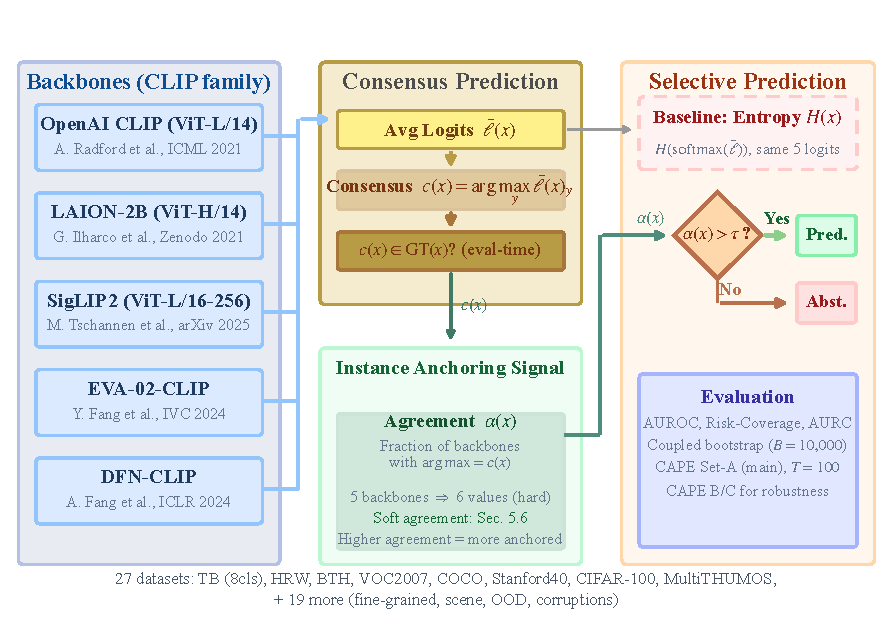
\includegraphics[width=\textwidth]{figures/fig1_method.pdf}
\caption{Pipeline for evaluating cross-model agreement as a confidence signal. Five CLIP-family backbones independently generate logits for an input image. Averaged logits produce a consensus prediction; the fraction of backbones voting for the consensus defines the agreement signal $\alpha(x)$ (hard agreement). The \emph{consensus-coordinate Jensen gap} (normalizing per-backbone softmaxes before versus after averaging) measures cross-backbone shape divergence and predicts error on its own (AUROC 0.622); \emph{soft agreement} (mean softmax mass at the consensus class) is the confidence-scoring function built on this gap. At inference, images below a threshold $\tau$ are abstained. Both signals are compared against compute-matched ensemble entropy, MSP, and margin across the 27 benchmark datasets of \S\ref{sec:datasets}.}
\label{fig:method}
\end{figure}

\subsection{Instance-Level Anchoring}

Let the consensus prediction $\hat{y}_{\text{cons}}(x) = \arg\max \frac{1}{5}\sum_{b=1}^5 \ell_b(x)$.
Per-image correctness is $\mathbf{1}[\hat{y}_{\text{cons}}(x) \in \text{GT}(x)]$ (multi-label: any true class).

The \emph{instance anchoring} (agreement) signal is defined as
\begin{equation}
\alpha(x) = \frac{1}{5}\sum_{b=1}^5 \mathbf{1}[\arg\max \ell_b(x) = \hat{y}_{\text{cons}}(x)],
\label{eq:agreement}
\end{equation}
the fraction of backbones voting for the consensus class.
$\alpha(x)$ takes discrete values $\{0.0, 0.2, 0.4, 0.6, 0.8, 1.0\}$.

\subsection{The plurality-induced ceiling}
\label{sec:ceiling}

\emph{This decomposition is descriptive: it reproduces the empirical wrong-consensus amplification; it does not predict whether agreement will carry signal on a new dataset.}

\paragraph{Why agreement can beat entropy.}
Agreement can outperform entropy on co-occurrence-ambiguous images for a specific reason. Entropy measures the dispersion of the average probability distribution, a single scalar. It does not distinguish two failure modes that CLIP exhibits under co-occurrence ambiguity: (i) genuine uncertainty, spreading probability across many classes, or (ii) high confidence in a wrong class that is a competing co-occurring label.
Agreement, by contrast, probes whether multiple diverse backbones converge on the same top-1 prediction.
When co-occurrence ambiguity is present (e.g., an image containing both \texttt{teacher} and \texttt{blackboard-writing}), different backbones may latch onto different equally-plausible labels, generating disagreement even when each backbone is individually confident.
Entropy cannot detect this failure mode because the average probability may appear sharp; agreement can, because each backbone votes differently.
This provides a plausible mechanism for why agreement can outperform entropy on some co-occurrence-ambiguous instances, but the cross-dataset experiments of \S\ref{sec:generalization} show that multi-label structure alone is insufficient (COCO and MultiTHUMOS tie or lose globally).

\paragraph{Two structural factors governing agreement.}
\label{sec:saturation}
This section characterizes why agreement carries discriminative signal in some regimes but not others.
Two structural factors jointly govern the information content of cross-model agreement; neither is a causal explanation, but together they delineate the regimes in which agreement can and cannot serve as a reliability signal.

\textbf{Factor 1: The plurality-induced ceiling.}
Even if backbone errors were completely independent, the multi-class voting procedure itself inflates agreement on wrong predictions.
Throughout, $p$ denotes the mean per-backbone accuracy, $p = \frac{1}{5}\sum_b \Pr(\arg\max \ell_b(x) \in \text{GT}(x))$, computed on the labeled evaluation set (Table~\ref{tab:saturation}).
Individual backbone accuracies are heterogeneous (e.g., on \tb{} they range from 0.459 to 0.855 with mean $0.67$; on MultiTHUMOS, SigLIP2 collapses to 0.030 vs~0.155--0.167 for the other backbones, giving mean $p{=}0.135$). The pooled mean $p$ is used in the $\kappa$ accounting, and the Monte Carlo simulations of Appendix~\ref{sec:kappa_decomp} use the empirical per-backbone accuracies $\{p_b\}$ rather than a homogeneous $p$.
Let each backbone independently classify an image correctly with probability $p$, and when incorrect, choose uniformly among the $C-1$ wrong classes.
Under this i.i.d.\ model, the expected per-image agreement on consensus-correct images approximates the per-backbone accuracy,
\begin{equation}
\mathbb{E}[\alpha \mid \text{correct}] \approx p,
\label{eq:alpha_correct}
\end{equation}
which holds asymptotically as $K \to \infty$ and empirically for moderate-to-large $C$ (e.g., \tb: $0.672$ vs~$p{=}0.67$; CIFAR-100: $0.772$ vs~$0.71$). For small $C$ combined with correlated backbones (\hrw, \bth), $\mathbb{E}[\alpha\mid\text{correct}]$ approaches its ceiling ($>0.9$) because correlated backbones move together. This pushes agreement toward 1 whenever the consensus is correct, a separate saturation mechanism discussed in Factor 2 below.
For wrong-consensus images, the marginal probability that a backbone votes a specific wrong class $w$ is $(1-p)/(C-1)$. Naively extending this to the conditional expectation $\mathbb{E}[\alpha \mid \text{wrong}]$ gives the i.i.d.\ baseline $\Delta_\alpha^{\text{iid}} = p - (1-p)/(C-1)$, which on \tb\ predicts a gap of $0.62$. However, the empirical gap is only $0.19$ (Table~\ref{tab:saturation}). On \hrw\ the i.i.d.\ prediction ($0.38$) is even further from the near-saturated empirical agreement (mean $0.903$, std $0.170$), and the empirical $\mathbb{E}[\alpha\mid\text{wrong}]$ is $0.825$, far above the i.i.d.\ predicted $0.21$ (the marginal rate $(1-p)/(C-1)$).
The failure of the i.i.d.\ baseline reflects that real backbone errors are correlated: backbones tend to confuse the same class pairs, inflating agreement on wrong-consensus images far above the marginal rate.

This is formalized with a \emph{wrong-consensus amplification} factor $\kappa \geq 1$, defined as the ratio of empirical $\mathbb{E}[\alpha \mid \text{wrong}]$ to the i.i.d.\ marginal rate:
\begin{equation}
\mathbb{E}[\alpha \mid \text{wrong}] \;=\; \kappa \cdot \frac{1-p}{C-1}, \qquad \kappa \;:=\; \frac{\mathbb{E}[\alpha \mid \text{wrong}]\,(C-1)}{1-p}.
\label{eq:kappa}
\end{equation}
The discriminative gap becomes
\begin{equation}
\Delta_\alpha = p - \kappa(1-p)/(C-1), \qquad p^\star = \frac{\kappa}{C-1+\kappa},
\label{eq:delta}
\end{equation}
where $p^\star$ is the accuracy at which the mean separation vanishes.
By construction, substituting Eq.~\eqref{eq:kappa} reduces the gap to the mean-agreement separation itself, $\Delta_\alpha = p - \mathbb{E}[\alpha \mid \text{wrong}]$: the parameterization is a re-expression of measured quantities, not an independent hypothesis.
Its mechanical content lies in the i.i.d.\ Monte Carlo reproduction of $\mathbb{E}[\alpha \mid \text{wrong}]$ (\S\ref{sec:kappa_decomp}), which attributes the bulk of the amplification to plurality-vote conditioning rather than to correlated errors.
$\kappa$ is \emph{not} a causal predictor: it aggregates plurality-vote conditioning together with deviation from i.i.d.\ backbone behavior (decomposed in \S\ref{sec:kappa_decomp}), of which the former is the dominant component.
It is used as an explanatory coordinate for analyzing observed regimes, rather than as a standalone criterion for selecting agreement before labels are available.
Classical majority-vote analysis \citep{hansen1990neural, lam1997application} characterized how ensemble error rates relate to member accuracies and correlations; $\kappa$ instead conditions on the consensus being wrong and quantifies how strongly agreement is amplified there. The classical quantities are majority-vote \emph{accuracy} and its dependence on member accuracies and pairwise correlations; $\kappa$ is a different functional, the \emph{agreement level} conditioned on the consensus error event, normalized by the i.i.d.\ marginal rate, and the decomposition of \S\ref{sec:kappa_decomp} further separates its plurality-vote and non-i.i.d.\ components. Neither classical theory conditions on wrong-consensus agreement, which is the quantity that determines whether agreement can separate correct from incorrect predictions.
Consequently $p^\star$ is a post-hoc characterization, not an ex-ante deployment rule.
It bears emphasizing that $\Delta_\alpha > 0$ is a necessary, not sufficient, condition. It states that correct-consensus images have higher mean agreement than wrong-consensus images, which is required for agreement to separate classes. The AUROC also depends on the conditional \emph{distributions} of $\alpha$ given correctness and on the competing entropy signal.
Phase-diagram outcomes reported below therefore never interpret a positive $\Delta_\alpha$ as a guarantee of agreement superiority.
Empirically (Table~\ref{tab:saturation}), $\kappa$ ranges from 2.6 (\bth, $C{=}2$) to 162 (CIFAR-100, $C{=}100$), and scales roughly with $C$.
The i.i.d.\ marginal rate ($\kappa{=}1$) dramatically underestimates the empirical conditional $\mathbb{E}[\alpha \mid \text{wrong}]$ on all datasets (e.g., marginal rate $0.05$ for \tb\ vs~empirical $0.49$; $0.003$ for CIFAR-100 vs~$0.47$); the $\kappa$-extended decomposition matches by construction.

Cross-validating against i.i.d.\ plurality-vote Monte Carlo (simulating $K{=}5$ independent backbones at matched per-backbone accuracies $\{p_b\}$ and class count $C$), plurality mechanics alone reproduces 54--108\% of empirical $\kappa$ across 27 datasets (e.g., \tb: $\kappa_{\text{iid-MC}}=9.4$ vs~$\kappa_{\text{emp}}=10.3$, 91\%; MultiTHUMOS: $17.9$ vs~$33.2$, 54\%; CIFAR-100: $112.4$ vs~$161.7$, 70\%; Appendix~\ref{tab:kappa_decomposition}).
Shares above 100\% (VOC2007: $\kappa_{\text{iid-MC}}=25.5$ vs~$\kappa_{\text{emp}}=23.6$; Stanford40: $56.2$ vs~$54.4$) mean the i.i.d.\ null slightly overpredicts the empirical amplification, a small negative residual; they are reported at face value rather than as literal additive contributions.
This indicates that the bulk of $\kappa$ reflects a mechanical effect of plurality voting, with deviations from i.i.d.\ backbone behavior (correlated errors or non-uniform confusion structure) contributing a secondary augmentation. Both effects scale with $C$, so the qualitative scaling pattern is robust, but $\kappa$ is not a pure index of error correlation.

The mechanism composition is family-conditional: on ensembles that share training data, correlated errors dominate the amplification (plurality share 32--33\%), as established empirically in the cross-family and 2$\times$2 replication of \S\ref{sec:nonclip}. The regime signature is revisited next.

\textbf{Factor 2: The regime paradox (inverted-U on \tb, regime dependence elsewhere).}
The plurality-induced ceiling explains why agreement's discriminative budget is structurally limited; it does not explain \emph{where} the remaining budget is spent.
On \tb, agreement's advantage over entropy follows an inverted-U across label multiplicity: it loses to entropy at both extremes and wins only in a narrow middle regime.
On easy images (high consensus accuracy, low ambiguity), all backbones agree on most images regardless of correctness; agreement saturates.
On extremely hard images (very low $p$, severe class imbalance, or heterogeneous backbone quality), the consensus drifts toward chance level and agreement carries no structure.
Only in a middle regime of moderate difficulty with \emph{systematic} cross-backbone confusion (shared class-confusability geometry) does disagreement become informative: backbones tend to make the same kinds of mistakes, but differ on which mistake they make on a given image, creating informative variance in the agreement signal.
No universal inverted-U is claimed across datasets; the robust statement is \emph{regime dependence} (\S\ref{sec:elimination}).

This regime dependence manifests concretely in the experiments.
On \tb, agreement's largest advantage is on images with 2--3 co-occurring ground-truth labels ($\Delta = +0.113$/$+0.119$ for the 2-/3-label strata, \S\ref{sec:mechanism}) and on low-anchor intent classes such as \texttt{answer} ($\Delta = +0.193$).
On single-label \tb{} images, agreement loses ($\Delta = -0.020$); on images with 4+ labels, entropy wins ($\Delta = -0.058$).
On MultiTHUMOS, the same gradient appears: agreement wins only at 4+ labels ($\Delta = +0.031$, 4.8\% of frames), ties at 3 labels, and loses on 1--2 label frames (global $\Delta = -0.044$, \S\ref{sec:generalization}).
The paradox is that agreement is most discriminative on exactly the hardest images where selective prediction is most needed, but this signal is confined to a regime that cannot be identified ex ante from $(p, C, \kappa)$ alone (LOO sign recovery 81.5\% at $n{=}27$; 88.9\% for soft, \S\ref{sec:elimination}).

Because $\kappa$ scales with both $C$ and $1/(1-p)$, high-accuracy and large-$C$ datasets keep a positive gap even while losing (CIFAR-10 and CIFAR-100 both have positive $\Delta_\alpha$ yet hard agreement loses there), underscoring that a positive gap is necessary, not sufficient. The boundary therefore \emph{characterizes} the observed regimes as a function of measurable dataset properties ($p$, $C$, $\kappa$); it does not by itself predict agreement wins on a new dataset, as the leave-one-dataset-out analysis of \S\ref{sec:elimination} confirms.

Figure~\ref{fig:saturation} visualizes this behavior: panel~(a) shows $\mathbb{E}[\alpha \mid \text{correct}]$ (black, $\approx p$) and $\mathbb{E}[\alpha \mid \text{wrong}]$ (colored, decreasing with $p$; magnitude increases with $\kappa$); panel~(b) shows the resulting gap $\Delta_\alpha$, whose zero-crossing $p^\star=\kappa/(C-1+\kappa)$ is marked by vertical dotted lines and shaded saturation regions ($p<p^\star$). At \tb{}'s operating point ($p=0.67$, $\kappa=10$), the gap is small but positive; at higher $p$ or $\kappa$ it collapses, marking the saturation regime.

\begin{figure}[t]
\centering
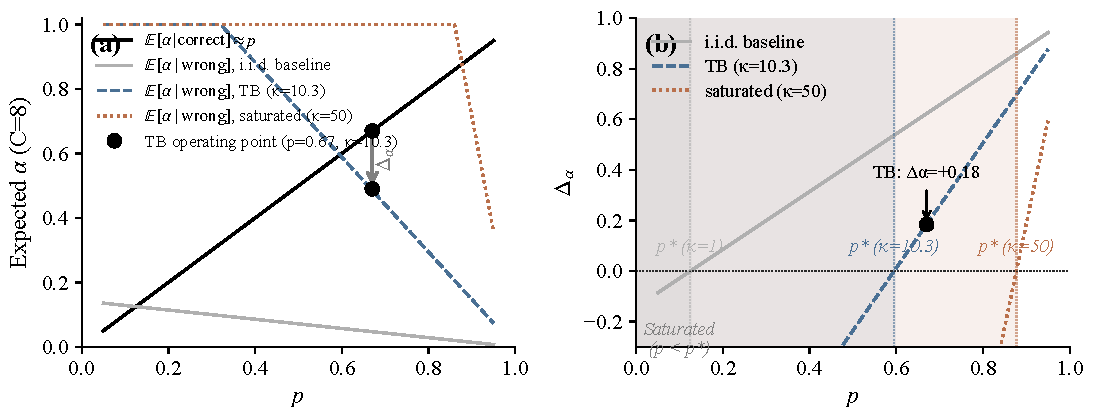
\includegraphics[width=0.85\textwidth]{figures/fig2_saturation.pdf}
\caption{Agreement saturation as a function of per-backbone accuracy $p$ ($C=8$, matching \tb). (a) Expected agreement conditioned on consensus correctness. (b) Discriminative gap $\Delta_\alpha$, with zero-crossing saturation threshold $p^\star = \kappa/(C-1+\kappa)$.}
\label{fig:saturation}
\end{figure}

\begin{table}[t]
\centering
\caption{Wrong-consensus amplification $\kappa$ across the eight datasets. $\kappa$ is defined as the ratio of empirical $\mathbb{E}[\alpha\mid\text{wrong}]$ to the i.i.d.\ marginal rate $(1-p)/(C-1)$. The threshold $p^\star = \kappa/(C-1+\kappa)$ marks the accuracy above which the mean agreement gap $\Delta_\alpha$ is positive; a positive gap is necessary, not sufficient, for agreement to outperform entropy (see \S\ref{sec:saturation}). $\kappa$ scales roughly with $C$; values are computed from per-image agreement on the labeled data and are not predicted ex ante.}
\label{tab:saturation}
\small
\begin{tabular}{lrrrrr}
\toprule
Dataset & $C$ & $p$ & $\kappa$ & $\mathbb{E}[\alpha\!\mid\!\text{wrong}]$ & $p^\star$ \\
\midrule
TeacherBehavior  & 8   & 0.67 & 10.3  & 0.487 & 0.60 \\
HandriseReadWrite & 3   & 0.59 & 4.0   & 0.825 & 0.67 \\
BowTurnHead      & 2   & 0.66 & 2.6   & 0.896 & 0.72 \\
VOC2007          & 20  & 0.69 & 23.6  & 0.379 & 0.55 \\
Stanford40       & 40  & 0.73 & 54.4  & 0.381 & 0.58 \\
COCO             & 80  & 0.69 & 97.7  & 0.388 & 0.55 \\
CIFAR-100        & 100 & 0.71 & 161.7 & 0.471 & 0.62 \\
MultiTHUMOS      & 65  & 0.13 & 33.2  & 0.449 & 0.34 \\
\bottomrule
\end{tabular}
\end{table}

\begin{table}[t]
\centering
\caption{Leave-one-dataset-out sign recovery of the boundary regression at $n{=}27$ under nested feature sets, reported with bootstrap CIs (B=10,000). \emph{C only} is a fully label-free prior; $p$ (per-backbone accuracy) requires labels; $\kappa$ is computed from labeled per-image agreement. The label-free control recovers at least as many signs as the full $(p,C,\kappa)$ refit, showing that sign recovery reflects a task prior rather than label-derived leakage. The two auxiliary rows replace empirical $\kappa$ with the i.i.d.\ plurality-MC baseline $\kappa_{\text{iid-MC}}$ (computed at $N{=}5\times 10^7$ on all 27 datasets).}
\label{tab:loocv_control}
\small
\begin{tabular}{lccccc}
\toprule
Features & \multicolumn{2}{c}{Hard agreement} & \multicolumn{2}{c}{Soft agreement} & \\
 & Sign acc & 95\% CI & Sign acc & 95\% CI & Label-free \\
\midrule
$C$ only              & 85.2\% & [70.4, 96.3] & 88.9\% & [77.8, 100.0] & yes \\
$p$, $C$              & 85.2\% & [70.4, 96.3] & 88.9\% & [77.8, 100.0] & no ($p$) \\
$p$, $C$, $\kappa$    & 81.5\% & [66.7, 96.3] & 88.9\% & [77.8, 100.0] & no ($p,\kappa$) \\
\midrule
$n{=}27$: $p$, $C$, $\kappa_{\text{iid-MC}}$ & 85.2\% & [70.4, 96.3] & 88.9\% & [77.8, 100.0] & no ($p$) \\
$n{=}27$: $p$, $C$, $\kappa$ (empirical)     & 81.5\% & [66.7, 96.3] & 88.9\% & [77.8, 100.0] & no ($p,\kappa$) \\
\bottomrule
\end{tabular}
\end{table}

\section{Experimental Setup}
\label{sec:setup}

\subsection{Datasets}
\label{sec:datasets}
The evaluation covers 27 datasets: the three \scbfive{} subsets (TeacherBehavior, 8 multi-label classes, 3,240 images; HandriseReadWrite, 3 classes, 1,671 images; BowTurnHead, 2 classes, 505 images) plus VOC2007 (20 classes, 2,510 images, multi-label), COCO (80 classes, 5,000 images, multi-label), Stanford40 (40 classes, 573 images), CIFAR-100 (100 classes, 10,000 images), and MultiTHUMOS (65 classes, 41,779 frames, multi-label).
The extension adds 19 benchmarks: Food-101, DTD, CIFAR-10, Tiny-ImageNet, STL-10, and EuroSAT (Hugging Face hub), SUN397, FGVC-Aircraft, Stanford-Cars, and GTSRB (ModelScope-recovered folder layouts), the out-of-distribution suite ImageNet-A, ImageNet-R, ImageNet-Sketch, ImageNet-V2 (matched, threshold, and top variants), and ImageNet-C, and the non-ImageNet corruptions CIFAR-10-C and CIFAR-100-C.
Per-image logits were extracted with five CLIP-family backbones under CAPE Set-A prompts (unscaled cosine similarities, temperature $T{=}100$), with the per-dataset image counts, class counts, and label types reported in Table~\ref{tab:meta_results}.
One dataset (Oxford-Flowers-102) was excluded because its mirror distribution carries a defective label-name mapping (class names replaced by ID strings; per-backbone accuracy at chance level, verified by feature inspection).
Three provenance deviations are disclosed: FGVC-Aircraft and Stanford-Cars use the official trainval/train splits as evaluation images (the test splits carry no public labels; no training occurs, so this introduces no label leakage, but it deviates from standard test-set reporting); GTSRB is evaluated from a ModelScope class-subdirectory mirror rather than the flat, CSV-annotated official test archive; and CIFAR-100-C is generated locally with the standard Hendrycks corruption transforms (about 105 images per corruption-severity combination) rather than taken from an official release, following the original corruption recipe. SUN397 and FGVC-Aircraft are covered as 61- and 90-class subsets of their official taxonomies, as reflected in Table~\ref{tab:meta_results}.
The cross-family and architecture-controlled cells reuse ImageNet-V2 matched/top and CIFAR-100 with the models evaluated in \S\ref{sec:nonclip}.

\subsection{Baseline Signals}

All baselines are compute-matched: they use the \emph{same} 5-backbone ensemble information.
\begin{itemize}
    \item \textbf{Ensemble entropy}: $-\sum_c p_c \log p_c$ where $p = \operatorname{softmax}(\frac{1}{5}\sum_b \ell_b / T)$.
    \item \textbf{MSP} (Maximum Softmax Probability): $\max_c p_c$, identified as the best overall CSF by Jaeger et al.\ \citep{jaeger2023call}.
    \item \textbf{Margin}: $\text{top}_1 - \text{top}_2$ of the averaged logits.
    \item \textbf{Logit variance}: negative of the mean across-backbone variance.
    \item \textbf{Class-level baselines}: \va{} AnchorScore (LAION-2B, from prior work) and a held-out 5-fold class-mean of agreement (fair class-level comparison).
    \item \textbf{Soft agreement}: $\alpha_{\text{soft}}(x) = \frac{1}{K}\sum_{k=1}^{K} p_k(y^* \mid x)$, where $y^*$ is the consensus class and $p_k(y \mid x) = \operatorname{softmax}(\ell_k(x) \cdot T)_y$ is backbone $k$'s softmax probability for class $y$ at temperature $T=100$.
    Unlike hard agreement, soft agreement retains the continuous degree of certainty: even when all backbones vote for the same class, their softmax probabilities for that class can differ, preserving discriminative information that hard agreement discards.
\end{itemize}

\subsection{Evaluation Protocol}

The evaluation follows standard selective prediction practice \citep{geifman2017selective, jaeger2023call}:
\begin{itemize}
    \item \textbf{AUROC} (area under receiver operating characteristic) for ranking quality, with coupled percentile bootstrap 95\% confidence intervals (B=10,000).
    \item \textbf{AUPR} (area under the precision-recall curve) for ranking quality under class imbalance.
    \item \textbf{AURC} (area under risk-coverage curve) for selective risk.
    \item \textbf{Selective accuracy} at fixed coverage points (30\%, 50\%, 70\%, 90\%).
    \item Because agreement is discrete (6 values), selective accuracy is reported with tie-aware randomization (200 seeds).
\end{itemize}

\section{Results}

\subsection{Main results on \scbfive{}}

On \tb{}, hard agreement is the best signal: it achieves AUROC 0.706, significantly outperforming entropy (0.639), MSP (0.652, Jaeger et al.'s best overall CSF), margin (0.662), and logit variance (0.536) (Table~\ref{tab:main}, which reports AUROC, AUPR, and AURC for all signals across all three subsets).
The coupled bootstrap $\Delta$ vs~entropy is $+0.067$ (95\%~CI~$[+0.052,+0.083]$).
The advantage is not an artifact of choosing the weakest baseline: agreement also significantly outperforms MSP ($\Delta = +0.054$, CI~$[+0.041,+0.067]$) and margin ($\Delta = +0.045$, CI~$[+0.030,+0.059]$), the strongest known baselines on \tb{} (Table~\ref{tab:main}).
A weighted variant that uses per-backbone Hit@1 as voting weights further sharpens the signal, but requires labeled validation data and is thus unavailable in zero-shot deployment (Appendix~\ref{sec:weighted}); the unweighted agreement is the relevant practical baseline and is used throughout the paper.

\begin{table}[t]
\centering
\caption{AUROC, AUPR, and AURC for all signals across three \scbfive{} subsets.
Hard agreement is the best signal on TeacherBehavior; entropy dominates on the easier subsets.
Bootstrap CIs (B=10,000).
For BowTurnHead (2 classes), entropy, MSP, and margin are monotonic transforms of $|p-0.5|$ and thus induce identical rankings, explaining the exact numerical agreement.}
\label{tab:main}
\small
\begin{tabular}{lcccc}
\toprule
Signal & AUROC & AUPR & AURC & $\Delta$ vs~entropy \\
\midrule
\multicolumn{5}{c}{\textbf{TeacherBehavior} (8cls, N=3240)} \\
\midrule
Entropy & 0.639 & 0.794 & 0.225 & --- \\
MSP & 0.652 & 0.803 & 0.218 & $+0.014$~$[+0.005,+0.023]$ \\
Margin & 0.662 & 0.807 & 0.215 & $+0.023$~$[+0.006,+0.039]$ \\
Hard agreement & \textbf{0.706} & \textbf{0.831} & \textbf{0.191} & $+0.067$~$[+0.052,+0.083]$ \\
Weighted agreement & 0.788 & 0.872 & 0.161 & $+0.149$~$[+0.133,+0.166]$ \\
Logit variance & 0.536 & 0.667 & 0.312 & $-0.103$~$[-0.127,-0.078]$ \\
\multicolumn{5}{c}{\textbf{HandriseReadWrite} (3cls, N=1671)} \\
\midrule
Entropy & \textbf{0.881} & 0.928 & 0.150 & --- \\
MSP & 0.880 & 0.927 & 0.150 & $-0.002$~$[-0.004,-0.000]$ \\
Margin & 0.877 & 0.926 & 0.151 & $-0.004$~$[-0.008,-0.001]$ \\
Hard agreement & 0.712 & 0.725 & 0.291 & $-0.170$~$[-0.185,-0.154]$ \\
Weighted agreement & 0.715 & 0.726 & 0.290 & $-0.166$~$[-0.182,-0.150]$ \\
Logit variance & 0.367 & 0.488 & 0.499 & $-0.514$~$[-0.547,-0.480]$ \\
\multicolumn{5}{c}{\textbf{BowTurnHead} (2cls, N=505)} \\
\midrule
Entropy / MSP / Margin\textsuperscript{*} & 0.580 & 0.715 & 0.270 & --- \\
Hard agreement & 0.536 & 0.743 & 0.252 & $-0.044$~$[-0.085,-0.004]$ \\
Weighted agreement & 0.540 & 0.757 & 0.240 & $-0.040$~$[-0.081,-0.000]$ \\
Logit variance & 0.552 & 0.745 & 0.259 & $-0.029$~$[-0.103,+0.045]$ \\
\bottomrule
\end{tabular}
\par
\vspace{4pt}
\begin{minipage}{\textwidth}\raggedright\footnotesize\textsuperscript{*}For 2-class problems, entropy, MSP, and margin are monotonic transforms of $|p-0.5|$ and thus yield identical rankings (hence identical AUROC/AUPR/AURC). Weighted agreement uses per-backbone Hit@1 as voting weights (Appendix~\ref{sec:weighted}); it is not a zero-shot baseline because the weights require a labeled validation set.\par\end{minipage}
\end{table}

Selective accuracy at 50\% coverage (tie-aware, 200 seeds) confirms the trend: hard agreement 78.52\% vs~entropy 74.63\%; at 70\% coverage: 71.96\% vs~67.68\%.
The risk-coverage curve (Figure~\ref{fig:riskcoverage}) shows hard agreement's advantage is concentrated in the low-coverage (high-precision) regime.

\begin{figure}[t]
\centering
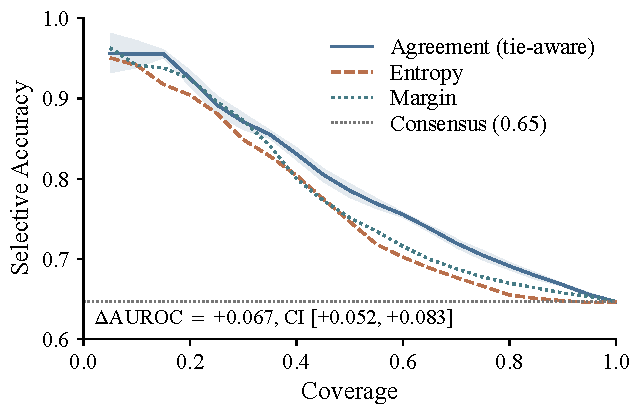
\includegraphics[width=0.48\textwidth]{figures/fig3_riskcoverage.pdf}
\caption{Risk-coverage curves on TeacherBehavior ($N{=}3{,}240$; tie-aware; agreement band = 2.5--97.5 percentiles across 200 tie seeds; entropy and margin baselines are shown for reference. Hard agreement achieves lower risk at every coverage level, with the largest gap in the low-coverage regime; the corresponding AUROC comparisons carry 95\% coupled bootstrap CIs (Table~\ref{tab:main}).}
\label{fig:riskcoverage}
\end{figure}

\paragraph{Per-class breakdown.}
The per-class advantage concentrates on the low-anchor class \texttt{answer} (Table~\ref{tab:perclass}, Figure~\ref{fig:mechanism}(c)): hard agreement 0.743 vs~entropy 0.550, $\Delta = +0.193$, contributing a substantial share of the headline gain. Excluding all \texttt{answer}-primary images (N=800 of 3240) drops the hard agreement vs~entropy gap from $+0.067$ to $+0.026$ (95\%~CI~$[+0.009,+0.044]$, still significant).
The gain is thus concentrated in, but not exclusive to, a single class: \texttt{guide} ($+0.062$), the other low-anchor class with meaningful error mass, and the 2--3-label stratum ($\S\ref{sec:mechanism}$) show the same direction.
On high-anchor classes (\texttt{blackboard-writing}, \texttt{teacher}), hard agreement and entropy perform similarly.

\begin{table}[t]
\centering
\caption{Per-class AUROC on TeacherBehavior (8 classes, N=3240). Agreement's largest advantage is on the low-anchor class \texttt{answer}.}
\label{tab:perclass}
\small
\begin{tabular}{lrrrrr}
\toprule
Class & $N$ & Acc & Entropy AUROC & Agreement AUROC & $\Delta$ \\
\midrule
guide & 372 & 0.570 & 0.519 & 0.581 & $+0.062$ \\
\textbf{answer} & \textbf{800} & \textbf{0.497} & \textbf{0.550} & \textbf{0.743} & \textbf{$+0.193$} \\
on-stage interaction & 141 & 0.943 & 0.827 & 0.711 & $-0.116$ \\
blackboard-writing & 235 & 0.974 & 0.918 & 0.913 & $-0.005$ \\
teacher & 1459 & 0.736 & 0.684 & 0.685 & $+0.001$ \\
stand & 169 & 0.219 & 0.483 & 0.501 & $+0.017$ \\
screen & 24 & 0.500 & 0.618 & 0.545 & $-0.073$ \\
\bottomrule
\end{tabular}
\par
\vspace{4pt}
\begin{minipage}{\textwidth}\raggedright\footnotesize\textsuperscript{*}blackboard (N=40) excluded: 0\% accuracy, AUROC undefined. Screen (N=24) has a small sample (CI not reported).\par\end{minipage}
\end{table}

\paragraph{Variant comparison.}
\label{sec:variants}
Alternate agreement operationalizations were tested on \tb\ and the seven other datasets.
Top-3 Jaccard similarity is dominated (AUROC 0.476). A continuous soft variant (each backbone's mean softmax probability on the consensus class) reaches 0.673 on \tb, slightly below hard agreement (0.706) but above entropy (0.639); it correlates with entropy ($r=+0.94$) because both depend on softmax sharpness.
However, the 27-dataset evaluation (\S\ref{sec:soft_agreement}) reveals that this soft variant, there called \emph{soft agreement}, generalizes far more broadly than either hard agreement or entropy: it outperforms entropy on 23 of 27 datasets, and its edge over MSP, the strongest known CSF, concentrates in OOD and multi-label benchmarks (\S\ref{sec:sota_csf}).
The temperature ($T=100$, matching CLIP's logit scale) is critical: at $T=1$, softmax probabilities are too flat to carry signal; at $T=100$, they capture cross-backbone distribution-shape divergence (the Jensen gap, \S\ref{sec:jensen_gap}).
On the original 8 datasets, soft agreement already exceeds hard agreement on 7 of 8 (the sole exception is \tb, 0.673 vs~0.706) and beats ensemble entropy on 5 of 8, but its full advantage is realized at scale (\S\ref{sec:soft_agreement}).
A Borda-count variant using each backbone's full ranking of the consensus class is more competitive on \tb\ (AUROC 0.712, $\Delta=+0.005$ vs~discrete, CI~$[-0.008,+0.019]$, not significant) but \emph{collapses} on datasets with larger $C$ (AUROC 0.15 on Stanford40, $C{=}40$; 0.33 on COCO, $C{=}80$), because Borda scores become noisy when the consensus class is ranked low by all backbones.
On the original 8 datasets, the discrete top-1 vote fraction is the most \emph{robust} hard-agreement operationalization: it is never significantly worse than alternative hard variants and avoids the large-$C$ instability of Borda.
(Whether hard or soft agreement is the better confidence signal is settled by the 27-dataset comparison in \S\ref{sec:sota_csf}, where soft agreement wins.)

\subsection{Mechanism analysis on TeacherBehavior}
\label{sec:mechanism}

\paragraph{Multi-label degree.}
On images with 2 or 3 true labels, agreement has its largest edge ($\Delta > +0.11$ AUROC).
On single-label images, both signals are weak ($\Delta \approx -0.02$).
On images with 4+ labels (typically high-anchor classes like \texttt{blackboard-writing}), entropy actually beats agreement ($\Delta = -0.058$).
This non-monotonic pattern shows the driver is not simply ``multi-label vs~single-label'' but rather the specific co-occurrence structure of low-anchor intent classes.

\paragraph{Anchor level.}
Stratifying by whether the \emph{primary} class is low- or high-anchor \citep{llm_annotation} (Figure~\ref{fig:mechanism}(a,b)):
low-anchor images (guide, answer, on-stage interaction, stand) have $\Delta = +0.127$; high-anchor images have $\Delta \approx 0.0$.
Hard agreement's entire advantage comes from low-anchor classes.
Removing \texttt{answer} (the single largest driver) reduces the low-anchor $\Delta$ from $+0.127$ to $+0.054$ (CI~$[+0.017,+0.091]$), and the gain survives on the remaining three classes, ruling out a single-class artifact.
The low-anchor partition is inherited from a different protocol (bbox-crop MLLM) and does not perfectly align with the per-class AnchorScore measured here (e.g., \texttt{on-stage interaction} is labeled ``low-anchor'' yet has a higher AnchorScore than some high-anchor classes); a quantitative redefinition is left for future work.

\paragraph{Complementarity with entropy.}
Spearman correlation between hard agreement and entropy is 0.715 on \tb.
Within the high-entropy half of images (where CLIP is most uncertain), hard agreement achieves AUROC 0.783, higher than its global 0.706.
A combined rank-sum signal does not beat hard agreement alone ($-0.025$ CI excluded 0), suggesting that entropy provides limited incremental information beyond hard agreement on this subset.

\paragraph{Saturation.}
On \hrw{}, where entropy dominates, hard agreement is near-saturated: mean 0.903, std 0.170 (Eq.~\eqref{eq:alpha_correct} at its ceiling).
On \tb{}, hard agreement is more variable: mean 0.607, std 0.255.
Hard agreement retains discriminative mean-separation only when it does not saturate.

\paragraph{Saturation along the prompt dimension.}
The saturation mechanism reproduces when the ensemble is expanded along a
second axis: the prompt set. Pooling the CAPE-A/B/C prompt sets (15 votes
per image instead of 5) raises \tb{} consensus accuracy from 64.7\% to
88.5\%, deepening saturation exactly as in the easy subsets, and entropy is
the larger beneficiary: entropy AUROC rises from 0.532 to 0.793
($+0.261$, 95\%~CI~$[+0.238,+0.285]$) while agreement rises from 0.591 to
0.730 ($+0.140$, CI~$[+0.111,+0.168]$), and at 15 votes agreement loses to
entropy ($\Delta = -0.063$, CI~$[-0.082,-0.044]$).
All signals here are evaluated against the 15-vote consensus correctness
(the same target for both vote counts); the 0.532 baseline is therefore
not directly comparable to Table~\ref{tab:main}'s 0.639, which targets the
5-vote consensus correctness.
On \hrw{} and \bth{}, prompt pooling does not rescue hard agreement: consensus accuracy is essentially unchanged (58.5\%$\rightarrow$59.9\% and 68.5\%$\rightarrow$67.5\%), and under the common 15-vote correctness target hard agreement still loses to entropy on \hrw{} ($\Delta = -0.063$, CI~$[-0.074,-0.052]$; agreement gains $+0.090$~CI~$[+0.069,+0.110]$ while entropy is essentially unchanged, $-0.004$~CI~$[-0.013,+0.004]$) and ties on \bth{} ($\Delta = -0.017$, CI~$[-0.056,+0.022]$).
The width axis (number of backbones), the prompt axis (number of prompt
sets), and the task-difficulty axis (easy vs~hard subsets) thus all trace
regime dependence rather than a single saturation curve: on \tb, prompt
pooling flips the edge in entropy's favor (from $+0.059$ to $-0.063$ under
the common 15-vote target), while on \hrw{} it narrows the loss
($-0.157$ to $-0.063$) and on \bth{} it leaves a tie.
Note that quantifying agreement to its vote grid ($\operatorname{round}(15\alpha)/15$
before rank statistics) is required here: naive averaging of the three
prompt sets introduces floating-point tie noise that perturbs the AUROC at
the $10^{-3}$ level.

\begin{figure}[t]
\centering
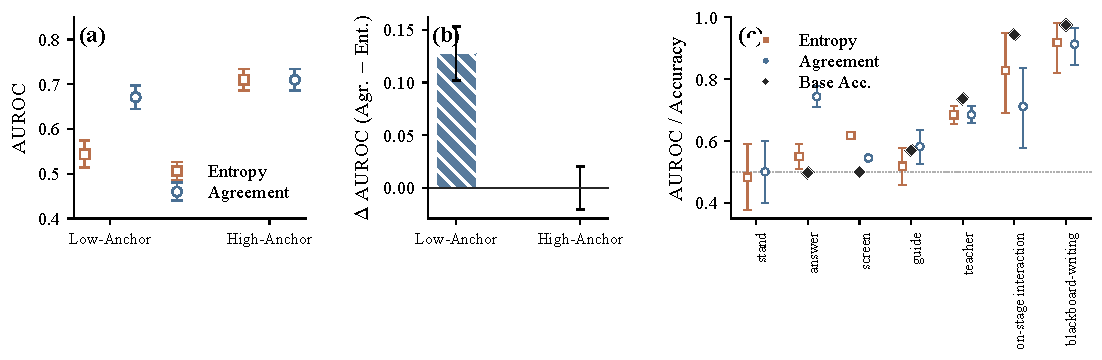
\includegraphics[width=0.99\textwidth]{figures/fig4_mechanism.pdf}
\caption{Mechanism analysis on TeacherBehavior ($N{=}3{,}240$). (a) AUROC by anchor level: agreement's advantage concentrates on low-anchor intent classes and vanishes on high-anchor classes. (b) AUROC delta (agreement $-$ entropy) by anchor level. (c) Per-class AUROC and consensus accuracy: the largest agreement advantage is on the low-anchor class \texttt{answer}. Error bars: 95\% coupled bootstrap CIs ($B{=}10{,}000$); \texttt{blackboard} omitted from (c) (degenerate: 0\% consensus accuracy, AUROC undefined).}
\label{fig:mechanism}
\end{figure}

\subsection{Instance-level vs~class-level anchoring}

Instance agreement is compared to two class-level baselines:
\begin{itemize}
    \item \va{} AnchorScore \citep{visualanchor} (per-class LAION-2B accuracy).
    \item Held-out class mean of per-instance agreement (5-fold cross-validation, fair comparison).
\end{itemize}

The result against the two class-level baselines is clear (Table~\ref{tab:classvsinstance}, Figure~\ref{fig:classvsinstance}): instance agreement significantly beats the \va{} AnchorScore ($\Delta = +0.055$, 95\%~CI~$[+0.030,+0.080]$).
The gap vs~the held-out class mean is smaller ($\Delta = +0.012$, CI straddles zero).
However, at the deployment-relevant low-coverage regime (30\% coverage), instance agreement clearly outperforms both class-level baselines (+5.8pp over held-out class mean, +10.4pp over \va{} AnchorScore).

Instance and class-level signals are complementary: the combined signal (instance + class mean) achieves AUROC 0.760, significantly better than instance alone ($+0.054$, 95\%~CI~$[+0.042,+0.066]$).

\begin{table}[t]
\centering
\caption{Instance vs~class-level anchoring on TeacherBehavior.
At low coverage (30\%), instance agreement clearly beats both class-level baselines.
Combined signal (instance + class mean) outperforms either alone.}
\label{tab:classvsinstance}
\small
\begin{tabular}{lccc}
\toprule
Signal & AUROC & Sel. Acc@30\% & Sel. Acc@50\% \\
\midrule
Instance agreement & \textbf{0.706} & \textbf{87.03\%} & 78.52\% \\
Class mean (held-out) & 0.695 & 81.26\% & 78.38\% \\
VA AnchorScore & 0.651 & 76.64\% & 75.13\% \\
Instance + class mean & \textbf{0.760} & --- & --- \\
\bottomrule
\end{tabular}
\par
\vspace{4pt}
\begin{minipage}{\textwidth}\raggedright\footnotesize\textsuperscript{*}Combined signal selective accuracy not computable from held-out class-mean protocol; AUROC confirms complementarity.\par\end{minipage}
\end{table}

\begin{figure}[t]
\centering
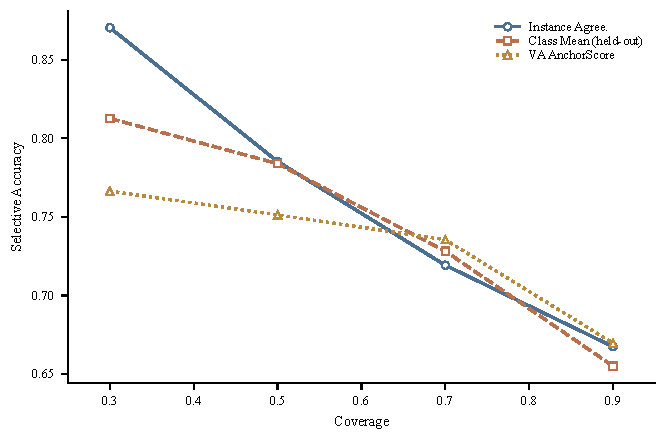
\includegraphics[width=0.85\textwidth]{figures/fig5_classvsinstance.pdf}
\caption{Instance-level vs~class-level anchoring on TeacherBehavior (selective accuracy, point estimates; comparison CIs in the text). Instance agreement outperforms both class-level baselines at low coverage (30\%). The combined two-level signal (instance $+$ class mean) is reported in Table~\ref{tab:classvsinstance}.}
\label{fig:classvsinstance}
\end{figure}

\subsection{Cost efficiency across backbone counts}

Agreement's advantage over entropy improves with $k$ and saturates around $k=4$ (Table~\ref{tab:cost}, Figure~\ref{fig:cost}).
At $k=2$, agreement AUROC (0.625) already exceeds single-backbone entropy (0.573), but this comparison is not compute-matched (2 vs~1 forward passes).
At matched compute ($k=2$ for both), agreement edges entropy on AUROC (0.625 vs~0.616) but entropy wins on selective accuracy at 30\% coverage (79.16\% vs~78.32\%).
Agreement's selective-accuracy advantage becomes consistent from $k \geq 3$; at $k=3$, agreement achieves 83.94\% vs~entropy 72.90\% at 30\% coverage (not compute-matched: this compares agreement@$k{=}3$ to entropy@$k{=}1$).
Performance improves with $k$, saturating around $k=4$.

Per-combination analysis shows the best 2-backbone pair is \texttt{openai + dfn} (agreement AUROC 0.688, $\Delta = +0.060$ vs~its 2-backbone ensemble entropy, CI~$[+0.044,+0.076]$), matching 5-backbone ensemble entropy (0.639; paired $\Delta = -0.004$, CI~$[-0.023,+0.015]$ on the full-ensemble consensus).
This is a cost saving rather than an accuracy gain: the pair reproduces the full ensemble's selective signal at two fifths of the compute.
Note: this is the best of $\binom{5}{2}=10$ pairs selected post hoc, and the effect size is post-selection (winner's-curse caveat).
Cross-dataset validation on all eight datasets confirms the caveat: \texttt{openai+dfn} beats its own 2-backbone entropy only on \tb\ ($+0.060$), and loses on the remaining seven (e.g., $-0.110$ on VOC2007, $-0.094$ on COCO, $-0.144$ on CIFAR-100; 95\%~CIs exclude zero), with no evidence of intrinsic cross-architecture complementarity.
Across all 10 pairs on \tb, the mean $\Delta$ is $+0.009 \pm 0.047$ (6/10 positive); the average 2-backbone benefit is modest, and openai+dfn is a favorable outlier.

\begin{table}[t]
\centering
\caption{Cost scaling on TeacherBehavior ($N{=}3{,}240$). Hard agreement AUROC as a function of $k$ backbones.
A 2-backbone agreement surpasses single-backbone entropy.}
\label{tab:cost}
\small
\begin{tabular}{lcccc}
\toprule
$k$ & $n$ subsets & Ensemble Ent AUROC & Agreement AUROC & Agr.\ Sel.\ Acc@30\% \\
\midrule
1 & 5 & 0.573 & --- & --- \\
2 & 10 & 0.616 & 0.625 & 78.32\% \\
3 & 10 & 0.634 & 0.675 & 83.94\% \\
4 & 5 & 0.637 & 0.699 & 85.23\% \\
5 & 1 & 0.639 & \textbf{0.706} & \textbf{87.08\%} \\
\bottomrule
\end{tabular}
\par
\vspace{4pt}
\begin{minipage}{\textwidth}\raggedright\footnotesize At $k{=}1$, agreement is undefined (single-backbone voting is trivial); ensemble entropy at $k{=}1$ achieves selective accuracy 72.90\%.\par\end{minipage}
\end{table}

\begin{figure}[t]
\centering
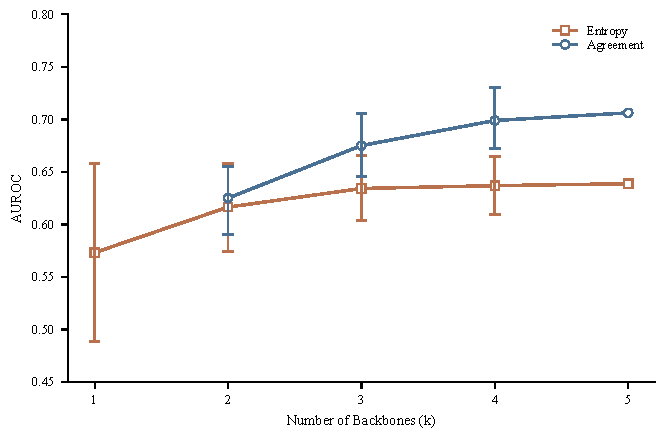
\includegraphics[width=0.85\textwidth]{figures/fig6_cost.pdf}
\caption{Cost scaling on TeacherBehavior ($N{=}3{,}240$; error bars: 95\% bootstrap CIs across backbone subsets). Hard agreement AUROC as a function of the number $k$ of backbones. 2-backbone agreement already surpasses single-backbone entropy (not compute-matched, 2 vs~1 forward passes); diminishing returns saturate at $k \approx 4$.}
\label{fig:cost}
\end{figure}

\subsection{Generalization to five additional datasets}
\label{sec:generalization}

To test whether hard agreement's advantage extends beyond \scbfive{}, the analysis was replicated on five additional datasets.
Figure~\ref{fig:generalization} shows risk-coverage curves across the four datasets where curves are available.

\paragraph{VOC2007 (20 classes, 2,510 images, 43.5\% multi-label).}
Hard agreement matches entropy ($\Delta = -0.007$, 95\%~CI~$[-0.021,+0.006]$).
MSP achieves 0.908, marginally outperforming both.
Unlike \tb, stratifying VOC2007 by multi-label degree does not reveal a hard agreement advantage: even on images with 2--3 ground-truth labels (1,040 images), hard agreement and entropy are indistinguishable ($\Delta = +0.003$, CI~$[-0.021,+0.025]$).

\paragraph{COCO (80 classes, 5,000 images, mean 2.9 labels/image).}
Overall, hard agreement and entropy are indistinguishable ($\Delta = +0.004$, CI~$[-0.009,+0.018]$).
Stratifying by multi-label degree shows a marginal hard agreement advantage on images with 2--3 labels ($\Delta = +0.024$, CI~$[+0.003,+0.046]$), far smaller than \tb's corresponding effect ($+0.113$).
As a further probe, COCO classes were grouped into semantic categories (vehicles, kitchenware, animals, furniture, electronics, sports equipment), and images containing $\geq$2 labels from the same category were analyzed.
None of these intra-category subsets showed a significant hard agreement advantage (e.g., vehicle: $\Delta = +0.028$, CI straddles zero; kitchenware: $\Delta = -0.018$).
Across both VOC2007 and COCO, the hard agreement advantage does not reproduce the magnitude or robustness of the TeacherBehavior effect: even the largest COCO stratum advantage ($+0.024$, CI~$[+0.003,+0.046]$) is only about a fifth of \tb's 2--3-label advantage, and the global COCO and VOC2007 effects are statistically indistinguishable from zero.

\paragraph{Stanford40 (40 classes, 573 images, single-label).}
Hard agreement slightly beats entropy ($\Delta = +0.039$, 95\%~CI~$[-0.017,+0.087]$, CI straddles zero) and MSP (0.923 vs~0.914).
Both signals are high (hard agreement 0.923, entropy 0.884).

\paragraph{CIFAR-100 (100 classes, 10,000 images, single-label).}
Hard agreement loses to entropy ($\Delta = -0.043$, 95\%~CI~$[-0.054,-0.033]$), while MSP achieves 0.905, outperforming both.
Consistent with Jaeger et al., MSP is the best single-model CSF on standard recognition; hard agreement only dominates in the hard multi-label regime.

\paragraph{MultiTHUMOS (65 classes, 41,779 frames, 42.5\% multi-label).}
To test whether a second dense multi-label dataset reproduces the TB advantage, the complete 5-backbone protocol was run on MultiTHUMOS \citep{yeung2018every}, a video-based dense multi-label action recognition benchmark.
Sampling 200 validation videos at 1~fps yields 41,779 frames annotated with 65 action classes (mean 1.44 labels per frame).
The class distribution is strongly imbalanced: label frequencies range from 8 to 8,720 frames (median 287, max/min ratio $1090\times$), with the top-10 classes accounting for 66.6\% of all labels, a severity consistent with shared confusion on the few frequent actions.
Hard agreement loses to entropy globally ($\Delta = -0.044$, 95\%~CI~$[-0.049,-0.038]$), apparently contradicting the TB advantage.
However, stratifying by multi-label degree reveals a previously obscured gradient: hard agreement consistently loses on single- and dual-label frames ($\Delta = -0.012$, 95\%~CI~$[-0.023,-0.000]$ and $\Delta = -0.051$, 95\%~CI~$[-0.059,-0.042]$ respectively), ties at 3 labels ($\Delta = -0.005$, 95\%~CI~$[-0.017,+0.008]$), and \textbf{wins} at 4 labels ($\Delta = +0.031$, 95\%~CI~$[+0.012,+0.051]$).
Critically, the frames where hard agreement wins (4+ labels) constitute only 4.8\% of the dataset; single- and dual-label frames dominate the global average.
This gradient (the advantage increases with multi-label degree) loosely tracks the TeacherBehavior finding that the gain concentrates on the 2--3 label subset (the multi-label core of an 8-class dataset).
The structural difference (MultiTHUMOS labels temporally alternate, TB labels spatially co-occur) is a post-hoc observation, not a portable predictor: it cannot be translated into a validation-set rule for identifying TB-like datasets ex ante.
As a robustness probe, the protocol was repeated without SigLIP2 (whose Hit@1 collapses to 3.0\% at the 320$\times$180 frame resolution, vs~15.5--16.7\% for the other backbones): the pooled accuracy $p$ rises from 0.135 to 0.161, but $\kappa$ rises from 33.2 to 41.8 and the saturation point $p^\star$ from 0.34 to 0.40, so MultiTHUMOS remains in the saturated regime (consensus accuracy 0.18 $< p^\star$) and hard agreement still loses ($\Delta = -0.033$, 95\%~CI~$[-0.038,-0.029]$).
The qualitative conclusion is unchanged: the entropy advantage does not depend on SigLIP2's degraded features.

These results confirm that agreement's advantage is not universal: it is absent from MultiTHUMOS globally even though that dataset shares TB's multi-label density property.
On standard recognition benchmarks, MSP, which Jaeger et al.\ identify as the best overall CSF, matches or exceeds both entropy and agreement; in these experiments the clearest agreement advantage occurs in a specific multi-label regime, but that regime cannot yet be characterized ex ante.
Figure~\ref{fig:phase} summarizes these outcomes as a regime map across 27 datasets; the descriptive analysis is given in \S\ref{sec:elimination}.

\paragraph{Baseline sensitivity and multiple comparisons.}
Across the 27 datasets, hard agreement significantly beats entropy on eight datasets (TeacherBehavior, ImageNet-A/R, ImageNet-C, ImageNet-Sketch, ImageNet-V2 $\times$3), ties on four, and loses on 15; soft agreement wins 23 and loses only 3 (all $|\Delta| < 0.015$; \S\ref{sec:soft_agreement}).
The same pattern holds against MSP (1 win, 3 ties, 4 losses).
Against margin the picture is slightly less one-sided because margin is itself a weak CSF on MultiTHUMOS (AUROC 0.630 vs~entropy 0.686 there): agreement edges margin on that dataset ($\Delta = +0.013$, CI~$[+0.008,+0.017]$) while still losing to entropy and MSP, so the global \tb{} advantage is the only one that holds across all three baselines.
The headline $\Delta = +0.067$ on \tb{} is therefore not an artifact of selecting a favorable baseline (Table~\ref{tab:main} reports the full baseline comparison on \tb), but the multiple-testing caveat applies: with eight independent dataset comparisons, one significant win is within the range of chance (expected $\approx 0.4$ false positives at $\alpha{=}0.05$), and no evidence is claimed beyond \tb{}.
Within \tb{}, the effect is robust to temperature ($T$ sweep, $\Delta$ range $+0.046$ to $+0.205$), prompt set (CAPE-A), circularity controls, and a leave-one-backbone-out analysis, all reported in \S\ref{sec:ablations}.

\begin{figure}[t]
\centering
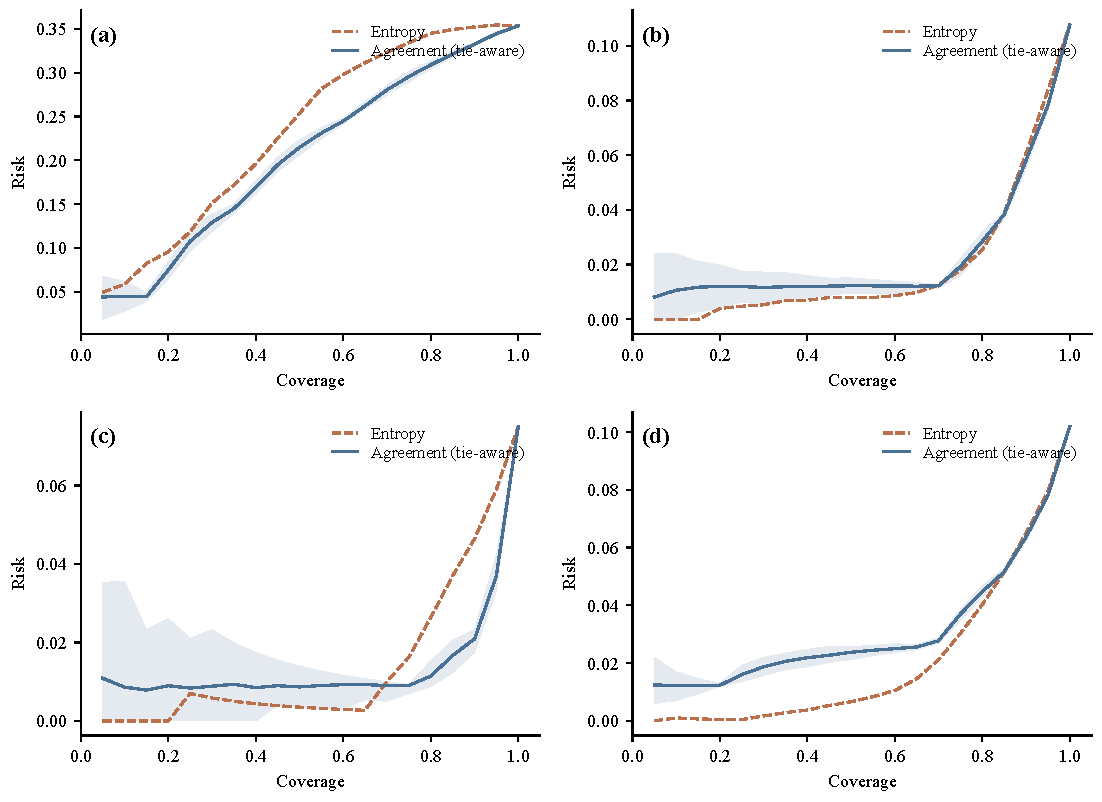
\includegraphics[width=\textwidth]{figures/fig7_generalization.pdf}
\caption{Risk-coverage curves for four datasets (tie-aware; agreement bands = 2.5--97.5 percentiles across 200 tie seeds; $N$ per dataset in Table~\ref{tab:meta_results}; AUROC comparison CIs in Table~\ref{tab:meta_results}; the COCO and MultiTHUMOS analyses report AUROC deltas and selective-accuracy points rather than curves, $\S\ref{sec:generalization}$): (a) TeacherBehavior, (b) VOC2007, (c) Stanford40, (d) CIFAR-100. Agreement beats entropy on TeacherBehavior ($\Delta = +0.067$), matches on VOC2007 ($\Delta = -0.007$), narrowly edges on Stanford40 ($\Delta = +0.039$, CI straddles zero), loses on CIFAR-100 ($\Delta = -0.043$). COCO ($\Delta = +0.004$) and MultiTHUMOS ($\Delta = -0.044$) are reported in the text; see Figure~\ref{fig:phase} for the full 27-dataset regime summary.}
\label{fig:generalization}
\end{figure}

\begin{figure}[t]
\centering
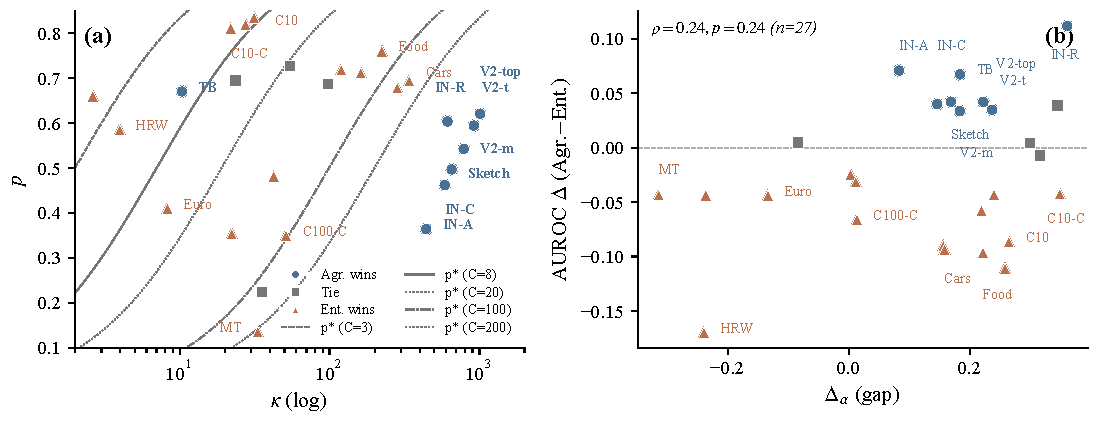
\includegraphics[width=0.95\textwidth]{figures/fig8_phase.pdf}
\caption{Regime map for cross-model agreement (27 datasets). \textbf{Left:} Each dataset plotted by $\kappa$ and per-backbone accuracy $p$; outcome (agreement wins, ties, or entropy wins) indicated by marker (the 16 datasets discussed in the text are labelled). Curves show $p^\star = \kappa/(C-1+\kappa)$ for selected $C$. Datasets above their $p^\star$ curve lie in the unsaturated regime. \textbf{Right:} Theoretical gap $\Delta_\alpha = p - \kappa(1-p)/(C-1)$ vs~empirical AUROC $\Delta$. The eight hard-agreement wins (TB and the seven ImageNet-family OOD benchmarks) all fall in the positive-gap region. The all-27-dataset correlation (Spearman $\rho = 0.24$) is weaker than the in-sample $n{=}8$ value discussed in \S\ref{sec:elimination}, consistent with the boundary's descriptive rather than predictive character.}
\label{fig:phase}
\end{figure}

\subsection{Soft agreement across 27 datasets}
\label{sec:soft_agreement}

The negative characterization above concerns \emph{hard} agreement (top-1 vote fraction, Eq.~\eqref{eq:agreement}).
This section evaluates \emph{soft agreement}, the mean softmax probability mass at the consensus class, and extends the evaluation from 8 to 27 datasets (adding 19 benchmarks: Food-101, DTD, CIFAR-10, Tiny-ImageNet, STL-10, EuroSAT, SUN397, FGVC-Aircraft, Stanford-Cars, GTSRB, the out-of-distribution suite ImageNet-A, ImageNet-R, ImageNet-Sketch, ImageNet-V2 (matched/threshold/top variants), ImageNet-C, and the non-ImageNet corruptions CIFAR-10-C and CIFAR-100-C; see \S\ref{sec:datasets} for provenance and exclusions).

Soft agreement beats entropy on 23 of 27 datasets, versus 8 of 27 for hard agreement (1 tie, 3 small losses with $|\Delta| < 0.015$; Table~\ref{tab:meta_results}, Figure~\ref{fig:win_comparison}).
The comparison against entropy is one axis of the evaluation only: \S\ref{sec:sota_csf} benchmarks soft agreement against seven additional CSFs (including MSP, energy, and ensemble mutual information), where it emerges as the best overall CSF.
\begin{itemize}
    \item Hard agreement wins 8 of 27 (TeacherBehavior +0.067, ImageNet-A +0.071, ImageNet-R +0.112, ImageNet-C +0.040, ImageNet-Sketch +0.042, ImageNet-V2-matched +0.034, ImageNet-V2-threshold +0.042, ImageNet-V2-top +0.035), all in the unsaturated regime ($p > p^\star$).
    \item \textbf{Soft agreement wins 23 of 27} (1 tie, 3 small losses with $|\Delta| < 0.015$) and never loses to energy or prediction variance (27/27 each) or to ensemble MI (26 wins, 1 tie).
    \item Soft agreement's wins span regimes: it wins on datasets where hard agreement ties or loses (Food-101 +0.020, CIFAR-10 +0.006, Stanford40 +0.089, EuroSAT +0.076) and on the unsaturated ImageNet-family OOD benchmarks (ImageNet-A +0.094, ImageNet-R +0.134, ImageNet-C +0.082, ImageNet-Sketch +0.094); it also wins on both non-ImageNet corruptions (CIFAR-10-C +0.008, CIFAR-100-C +0.007) where hard agreement loses.
\end{itemize}

\begin{figure}[t]
\centering
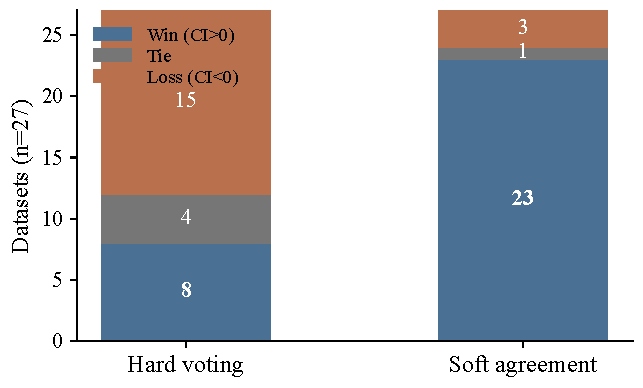
\includegraphics[width=0.5\textwidth]{figures/fig9_win_comparison.pdf}
\caption{Win-loss comparison across 27 datasets ($B{=}10{,}000$ coupled bootstrap; win = CI excludes 0). Hard agreement wins only 8 of 27; soft agreement wins 23 of 27 with 3 small losses.}
\label{fig:win_comparison}
\end{figure}

\begin{table}[t]
\centering
\caption{Agreement signals vs~entropy across 27 datasets ($B{=}10{,}000$ coupled bootstrap; win = CI excludes 0).}
\label{tab:meta_results}
\small
\begin{tabular}{lrrrrrlrrr}
\toprule
Dataset & $N$ & $C$ & $p$ & acc & $\kappa$ & $\Delta_{\text{hard}}$ & $\Delta_{\text{soft}}$ & H & S \\
\midrule
imagenet-r         & 10,000 & 1000 & 0.604 & 0.697 &  612 & $+0.112$ & $+0.134$ & W & W \\
imagenet-a         &  7,500 & 1000 & 0.364 & 0.437 &  441 & $+0.071$ & $+0.094$ & W & W \\
imagenet-v2-top    & 10,000 & 1000 & 0.621 & 0.765 & 1012 & $+0.035$ & $+0.095$ & W & W \\
imagenet-v2-threshold & 10,000 & 1000 & 0.594 & 0.733 & 916 & $+0.042$ & $+0.097$ & W & W \\
imagenet-v2-matched & 10,000 & 1000 & 0.543 & 0.670 & 785 & $+0.034$ & $+0.085$ & W & W \\
imagenet-sketch    & 10,000 & 1000 & 0.497 & 0.618 & 652 & $+0.042$ & $+0.094$ & W & W \\
imagenet-c         & 10,000 & 1000 & 0.462 & 0.599 & 586 & $+0.040$ & $+0.082$ & W & W \\
stanford40         &    573 &   40 & 0.726 & 0.925 & 54.4 & $+0.039$ & $+0.089$ & T & W \\
eurosat            &  2,700 &   10 & 0.409 & 0.541 &  8.3 & $-0.044$ & $+0.076$ & L & W \\
coco               &  5,000 &   80 & 0.687 & 0.894 & 97.7 & $+0.004$ & $+0.045$ & T & W \\
fgvc-aircraft      &  5,000 &   90 & 0.225 & 0.354 & 35.4 & $+0.005$ & $+0.036$ & T & W \\
teacher-behavior   &  3,240 &    8 & 0.670 & 0.647 & 10.3 & $+0.067$ & $+0.035$ & W & W \\
dtd                &  1,880 &   47 & 0.481 & 0.672 & 42.4 & $-0.025$ & $+0.028$ & L & W \\
food101            & 10,000 &  101 & 0.759 & 0.942 &  223 & $-0.097$ & $+0.020$ & L & W \\
voc2007            &  2,510 &   20 & 0.695 & 0.892 & 23.6 & $-0.007$ & $+0.019$ & T & W \\
cifar100           & 10,000 &  100 & 0.711 & 0.898 &  162 & $-0.043$ & $+0.019$ & L & W \\
stanford-cars      &  8,000 &  196 & 0.693 & 0.941 &  340 & $-0.094$ & $+0.013$ & L & W \\
gtsrb              & 10,000 &   43 & 0.353 & 0.464 & 22.2 & $-0.032$ & $+0.010$ & L & W \\
tiny-imagenet      & 10,000 &  200 & 0.678 & 0.795 &  283 & $-0.058$ & $+0.008$ & L & W \\
sun397             & 10,000 &   61 & 0.718 & 0.877 &  119 & $-0.090$ & $+0.006$ & L & W \\
cifar10            & 10,000 &   10 & 0.819 & 0.988 & 27.5 & $-0.087$ & $+0.006$ & L & W \\
cifar10c           & 10,000 &   10 & 0.810 & 0.935 & 21.9 & $-0.043$ & $+0.008$ & L & W \\
cifar100c          & 10,000 &  100 & 0.349 & 0.489 & 51.1 & $-0.066$ & $+0.007$ & L & W \\
stl10              &  8,000 &   10 & 0.834 & 0.993 & 31.3 & $-0.111$ & $+0.001$ & L & T \\
multithumos        & 41,779 &   65 & 0.135 & 0.183 & 33.2 & $-0.044$ & $-0.006$ & L & L \\
bow-turnhead       &    505 &    2 & 0.659 & 0.685 &  2.6 & $-0.044$ & $-0.012$ & L & L \\
handrise-readwrite &  1,671 &    3 & 0.585 & 0.585 &  4.0 & $-0.170$ & $-0.014$ & L & L \\
\midrule
\multicolumn{6}{r}{Win (CI$>$0)} & & & 8 & 23 \\
\multicolumn{6}{r}{Tie} & & & 4 & 1 \\
\multicolumn{6}{r}{Loss (CI$<$0)} & & & 15 & 3 \\
\bottomrule
\end{tabular}
\end{table}

All seven ImageNet-family out-of-distribution benchmarks (ImageNet-A, ImageNet-R, ImageNet-C, ImageNet-Sketch, and the three ImageNet-V2 variants) are natural instances of the unsaturated regime (all have $p > p^\star$ with large $\kappa$ and $C{=}1000$), confirming that TeacherBehavior is not a singleton but a class of benchmarks where hard agreement also wins.
The two non-ImageNet corruptions (CIFAR-10-C, $C{=}10$; CIFAR-100-C, $C{=}100$) are \emph{also} in the unsaturated regime by the $\kappa$-boundary criterion ($p = 0.810 > p^\star = 0.708$ and $p = 0.349 > p^\star = 0.341$), yet hard agreement still loses to entropy there ($-0.043$ and $-0.066$), underscoring that the $\kappa$-boundary is one-directional (saturated datasets never win; unsaturated datasets may still lose), while soft agreement still edges entropy on both ($+0.008$ and $+0.007$), so its advantage over entropy is not confined to the ImageNet family.

A leave-one-dataset-out evaluation at $n{=}27$ gives:
the theoretical $\Delta_\alpha$ sign rule recovers 48.1\% (13/27; CI~$[29.6,66.7]$, at chance with the extended suite);
the joint $(p,C,\kappa)$ refit recovers 81.5\% (22/27; CI~$[66.7,96.3]$) for hard agreement and 88.9\% (24/27; CI~$[77.8,100.0]$) for soft agreement.
Because $\kappa$ is computed from the labeled evaluation set, this LOO exercise is a \emph{label-conditional calibration check}, not an ex-ante prediction.
To isolate how much of the recovery depends on label-derived information, the identical protocol is run on nested feature sets (Table~\ref{tab:loocv_control}): using only the class count $C$, a fully label-free prior, recovers 85.2\% of signs for hard agreement and 88.9\% for soft agreement; adding $p$ leaves both unchanged; adding $\kappa$ changes hard agreement to 81.5\%.
The sign recovery is therefore driven by a task prior ($C$) rather than by the label-derived $\kappa$: the joint refit's accuracy does not reflect circular label leakage.
This is the mechanism corroborating itself rather than $\kappa$ failing: the class count is the plurality driver, so a $C$-only baseline recovering the signs is the ceiling's own signature.
The value of the $\kappa$ analysis lies in the \emph{decomposition}, not the raw $\kappa$: it separates plurality-dominated from correlation-dominated ensembles (the 2$\times$2 of \S\ref{sec:nonclip}) and quantifies the mechanical share of the amplification.
At $n{=}27$, both the joint refit and the $C$-only control exclude 50\% in their lower CI (unlike the $n{=}8$ evaluation where the CIs straddled chance), providing the first evidence that the boundary has modest out-of-sample calibration utility; the zero-parameter $\Delta_\alpha$ rule alone does not survive the larger suite.

\subsection{Cross-family replication and the 2$\times$2 mechanism split}
\label{sec:nonclip}
The CLIP family varies training \emph{data} as well as architecture. This dilutes error correlation relative to an ensemble that shares training data. Shared training data could in principle drive $\kappa$ through correlated errors rather than plurality mechanics.
To separate the two, the decomposition is replicated on a five-model ImageNet-supervised ensemble that \emph{shares} training data (ResNet-50, ViT-B/16, ConvNeXt-B, Swin-B, EfficientNet-B4; all ImageNet-1k) on ImageNet-V2 matched/top, contrasting with the CLIP family on the same datasets.
The amplification phenomenology replicates and intensifies: $\kappa_{\text{emp}}$ is 3.1--4.3$\times$ the CLIP value (2407 vs~785 on matched; 4383 vs~1012 on top), with $\mathbb{E}[\alpha\mid\text{wrong}]$ reaching 0.68--0.73, and hard agreement \emph{loses} to entropy on both ($-0.030$, CI $[-0.038,-0.022]$; $-0.041$, CI $[-0.053,-0.030]$) despite marginally positive $\Delta_\alpha$, consistent with the boundary's one-directionality.
But the decomposition inverts: plurality mechanics accounts for only 32--33\% of $\kappa$ (CLIP at the same $C{=}1000$: 73--88\% on ImageNet-A/R); the dominant share (67--68\%) is correlated error, consistent with the family's shared training data.
This attribution is descriptive rather than causal: the two families co-vary on three axes: training data (shared ImageNet-1k vs~five distinct web-scale sources), training objective (cross-entropy vs~contrastive), and architecture mix, so \emph{shared data} is a candidate driver, not an isolated variable.
The ceiling's \emph{existence} is therefore cross-model, while its \emph{mechanism} is family-conditional: data-diverse families saturate through plurality mechanics, data-shared families through error correlation; the $\kappa$ decomposition, computed from labeled per-image votes, distinguishes the two regimes empirically.
The shape-divergence signal survives the cross-family test: soft agreement beats entropy on both datasets ($+0.037$, CI $[+0.034,+0.041]$; $+0.051$, CI $[+0.046,+0.057]$) at roughly half the CLIP magnitude, and even retains a narrow but significant edge over MSP ($+0.004$, $+0.003$; both CIs exclude zero).
Caveats: the non-CLIP ensemble sits at a higher operating point on V2 ($p{=}0.718/0.834$ vs~CLIP's $0.543/0.621$; the decomposition matches per-backbone accuracies in simulation, but the AUROC deltas are not operating-point-matched), and softmax signals use $T{=}1$ on raw logits (vs~$T{=}100$ on cosine similarities; hard-vote and $\kappa$ metrics are temperature-free).

To extend the cross-family test beyond the ImageNet family, the same five ImageNet-supervised models are evaluated on CIFAR-100 with the 1000-class head restricted to the 63 CIFAR classes that have a defensible ImageNet-1k counterpart (the remaining 37 classes, e.g., baby, dinosaur, forest, orchid, have no ImageNet-1k class; the mapping is documented in the released code).
At this non-ImageNet operating point the ensemble is substantially weaker ($p{=}0.527$, consensus 0.573), yet the mechanism split persists: plurality share 45\% ($\kappa_{\text{emp}}$ = 84.9 vs~$\kappa_{\text{iid}}$ = 38.3), hard agreement loses to entropy ($-0.038$, CI~$[-0.049,-0.027]$), and soft agreement again beats entropy ($+0.032$, CI~$[+0.029,+0.036]$).
Notably, soft agreement also retains a narrow but significant edge over MSP ($+0.010$, CI~$[+0.008,+0.011]$): the claim that soft agreement's MSP edge is confined to ImageNet-family conditions therefore holds for the CLIP panel but not universally, and the panel-dependence is stated explicitly.

To isolate which family axis drives this mechanism split, the analysis completes a partial 2$\times$2 that crosses training-data diversity with architecture mix (cell A: the arch-diverse CLIP panel above; cell B: the shared-data ImageNet ensemble above) by adding a third cell (C) that holds \emph{architecture} fixed while varying training data: five ViT-B/32 backbones trained on five distinct web-scale datasets (OpenAI WIT-400M, LAION-400M, LAION-2B, DataComp-XL, CommonPool-M) on CIFAR-100 ($C{=}100$), where the arch-diverse CLIP cell has a committed reference (share 72\%).
With architecture fixed, plurality mechanics remains the dominant mechanism (share 59\%, $\kappa_{\text{emp}}=158.7$ vs~$\kappa_{\text{iid}}=94.0$), and the phenomenology reproduces: hard agreement loses to entropy ($-0.040$, CI $[-0.047,-0.034]$), soft agreement beats entropy ($+0.009$, CI $[+0.006,+0.012]$) while narrowly losing to MSP ($-0.005$), consistent with the MSP edge being confined to ImageNet-family OOD conditions.
The attribution therefore survives an architecture-controlled contrast: the data-sharing drop (72\%$\rightarrow$32--33\%) is far larger than the architecture modulation (72\%$\rightarrow$59\%), supporting \emph{training-data diversity} as the primary driver of the mechanism split with architecture mix as a secondary modulator (descriptive, not causal; the cells co-vary training objective and dataset family as well).
The fourth cell (D) holds architecture fixed on the data-shared side: five ViT-B/16 checkpoints with ImageNet-1k classification heads, varying only the training recipe (torchvision ViT-B/16, timm augreg-IN1k, augreg-IN21k$\rightarrow$IN1k, augreg2-IN21k$\rightarrow$IN1k, and orig-JFT/IN21k$\rightarrow$IN1k), evaluated on ImageNet-V2 matched.
Cell D reproduces cell B's mechanism mix: plurality share 34\% ($\kappa_{\text{emp}}=2283$ vs~$\kappa_{\text{iid}}=782$), hard agreement loses to entropy ($-0.061$, CI~$[-0.068,-0.054]$), and soft agreement again beats entropy ($+0.011$, CI~$[+0.009,+0.014]$) while essentially tying MSP ($-0.002$, CI just touching zero).
The 2$\times$2 is therefore complete on two dataset anchors: fixing the architecture barely moves the plurality share within either data regime (A$\rightarrow$C on CIFAR-100: 72\%$\rightarrow$59\%; B$\rightarrow$D on ImageNet-V2: 32--33\%$\rightarrow$34\%), while moving from data-diverse to data-shared flips the dominant mechanism regardless of architecture (A$\rightarrow$B: 72\%$\rightarrow$32--33\%; C$\rightarrow$D: 59\%$\rightarrow$34\%).

A further cell isolates the seed axis directly: five ResNet-18 classifiers trained from scratch on CIFAR-100 with different random seeds (identical architecture, data, protocol, and hyperparameters, the canonical deep-ensemble setting; 200 epochs, SGD with cosine schedule, batch 128, weight decay $5\times 10^{-4}$, test top-1 0.784--0.791 across seeds) reproduce the correlation-dominated mix (plurality share 46\%, $\kappa_{\text{emp}}=308$ vs~$\kappa_{\text{iid}}=142$), hard agreement loses to entropy ($-0.055$, CI~$[-0.064,-0.047]$), and soft agreement beats entropy ($+0.011$, CI~$[+0.010,+0.013]$) while tying MSP ($-0.000$, CI straddling zero).
Even the purest disagreement source (sampling variance alone) therefore reproduces both the ceiling's phenomenology and the shape-divergence signal's survival.



\subsection{The consensus-coordinate Jensen gap}
\label{sec:jensen_gap}
Soft agreement retains signal where hard agreement saturates because it normalizes \emph{before} averaging the backbones' logits; MSP normalizes \emph{after} averaging.
MSP computes $\operatorname{softmax}(\bar{z})_{y^*}$; it normalizes \emph{after} averaging the backbones' logits.
Soft agreement computes $\frac{1}{K}\sum_k \operatorname{softmax}(z_k)_{y^*}$; it normalizes \emph{before} averaging.
By Jensen's inequality, these differ whenever the backbones disagree about the distribution shape (not just the argmax).
The full difference is the vector gap
\begin{equation}
\operatorname{softmax}(\bar{z}) - \frac{1}{K}\sum_k \operatorname{softmax}(z_k),
\label{eq:jensen_gap}
\end{equation}
and its consensus-class coordinate, the scalar quantity $|\alpha_{\text{soft}} - \text{MSP}|$, is the \emph{consensus-coordinate Jensen gap}.
By construction, soft agreement and MSP differ exactly by this coordinate: the gap is not an auxiliary statistic but the identity linking the two scores, so soft agreement's edge over MSP is definitionally carried by the shape divergence the gap measures (the win record of \S\ref{sec:sota_csf} quantifies when that divergence adds signal).

The consensus-coordinate Jensen gap is non-zero on all 27 datasets (mean 0.027--0.21) and predicts per-image error on its own: its mean AUROC as an error detector is 0.622 (range 0.30--0.87), above chance on 22 of 27 datasets.
A mutual-information decomposition confirms the hierarchy: $I(\alpha_{\text{soft}}; \text{correct}) = 0.162 > I(\text{MSP}; \text{correct}) = 0.132 > I(\text{entropy}; \text{correct}) = 0.121$ (means across 27 datasets).
Soft agreement carries more information about correctness than either MSP or entropy because it preserves the per-backbone distribution-shape divergence (Eq.~\eqref{eq:jensen_gap}) that MSP normalizes away.
This construction is a sibling of the mutual-information epistemic-uncertainty decomposition \citep{houlsby2011bald}: both are Jensen gaps, the former on the entropy functional and the latter on the probability-mass functional, and the mutual-information hierarchy above quantifies the information each variant retains. The novelty is accordingly the empirical finding---that this gap predicts per-image error on its own and that the soft agreement built on it carries the CSF record of \S\ref{sec:sota_csf}---not the identity itself, which belongs to the BALD/MI lineage.
On datasets where all backbones agree on the argmax but differ in confidence (the saturated regime for hard agreement), this divergence can provide discriminative information that hard agreement discards; soft agreement captures it while hard agreement and MSP do not.


\subsection{Controlled co-occurrence manipulation}
\label{sec:cooccurrence_manip}

A synthetic experiment tests whether input-level visual co-occurrence is the causal driver of hard agreement's advantage, rather than label-set bookkeeping alone.
Two manipulation axes are applied to CIFAR-100 (single-label; hard agreement loses, $\Delta_{\text{hard}} = -0.043$) and VOC2007 (multi-label; $\Delta_{\text{hard}} = -0.007$):

\textit{Axis 1: Label injection (negative control).}
Each image's ground-truth label set is expanded by $k{-}1$ randomly chosen classes, making correctness depend on a larger set.
If multi-labelness alone drives agreement, this should create an advantage.
It does not: across $k \in \{2,3,4\}$ on both datasets, $\Delta_{\text{hard}}$ is unchanged (CIFAR-100: $-0.044$ at $k{=}1$ vs~$-0.043$ at $k{=}4$; VOC2007: $-0.007$ vs~$-0.009$).
Pure label-set expansion is inert, confirming that the signal requires visual co-occurrence, not just label-set arithmetic.

\textit{Axis 2: Image-pair merging (co-occurrence proxy).}
Synthetic samples are created by averaging the per-backbone logits of $k$ independently drawn images, simulating an image containing $k$ co-occurring visual concepts.
The ground-truth label set is the union of the merged images' labels.
On CIFAR-100, merging $k{=}2$ images produces a significant agreement advantage ($\Delta_{\text{hard}} = +0.021$, CI~$[+0.002, +0.040]$); at $k{=}4$, the advantage reverses ($\Delta_{\text{hard}} = -0.107$, CI~$[-0.124, -0.091]$).
On VOC2007, the effect is stronger: $k{=}2$ gives $\Delta_{\text{hard}} = +0.042$ (CI~$[+0.009, +0.077]$), $k{=}3$ gives $+0.064$ (CI~$[+0.024, +0.102]$), and $k{=}4$ returns to near-zero ($-0.006$).
This inverted-U (emergence at $k{=}2{-}3$, recession at $k{=}4$) matches the TeacherBehavior stratum pattern ($+0.113$ at 2--3 labels, $-0.058$ at 4+ labels).

\textit{Limitation.}
Logit averaging is a linear proxy for visual co-occurrence; a real image with two objects produces non-linear feature interactions that averaging cannot capture.
The synthetic distribution differs from natural data (merged samples have unrealistically diverse content).
This is therefore presented as causal-direction evidence: co-occurrence in the input is \emph{consistent with} the agreement signal (the manipulation reproduces it, while label-set bookkeeping alone does not), not as a quantitative model of natural co-occurrence effects.


\subsection{Comparison with modern confidence-scoring functions}
\label{sec:sota_csf}
Beyond ensemble entropy, soft agreement is compared against seven CSFs spanning three families: standard baselines (MSP~\citep{hendrycks2017baseline}, margin), logit-space scores (max-logit~\citep{hendrycks2022scaling}, energy~\citep{liu2020energy}), ensemble-uncertainty measures (ensemble mutual information~\citep{smith2018understanding}, prediction variance), and hard agreement.
All are compute-matched (derived from the same 5-backbone logits).

In the CSF hierarchy, soft agreement sits at the top with MSP (soft agreement $\approx$ MSP $>$ margin $>$ entropy $>$ max-logit $\gg$ energy, ensemble MI, prediction variance; Table~\ref{tab:sota_csf}).
Soft agreement never loses to energy, ensemble MI, or prediction variance (27/27, 26/27, and 27/27 datasets, respectively); it beats entropy and max-logit on 23 of 27.
Its closest competitor is MSP (the best overall CSF identified by \citet{jaeger2023call}): soft agreement wins on 14/27, ties on 6, and loses on 7, but retains a positive mean advantage ($+0.023$ AUROC; one-sample permutation test over the 27 dataset-level deltas, $p=0.001$).

The advantage over MSP is not diffuse: it concentrates where cross-backbone divergence is informative (\S\ref{sec:jensen_gap}).
Stratifying the 27 datasets (an exploratory, post-hoc analysis), the OOD stratum contains 7 of the 14 wins: all seven ImageNet-family benchmarks (ImageNet-A $+0.076$, ImageNet-R $+0.100$, ImageNet-C $+0.049$, ImageNet-Sketch $+0.061$, ImageNet-V2-matched $+0.065$, ImageNet-V2-threshold $+0.070$, ImageNet-V2-top $+0.068$), while the two non-ImageNet corruptions give a tie (CIFAR-100-C $+0.001$) and a narrow loss (CIFAR-10-C $-0.002$); the multi-label stratum contributes 3 wins, 1 tie, 0 losses (TeacherBehavior $+0.021$, VOC2007 $+0.017$, COCO $+0.028$; MultiTHUMOS $-0.001$).
The remaining 14 standard single-label datasets give 4 wins, 4 ties, 6 losses, each loss small ($|\Delta| \le 0.020$): MSP retains a narrow edge exactly where backbones rarely disagree (high-accuracy, low-divergence settings), while soft agreement's Jensen gap adds signal where disagreement is real.
As a sensitivity check, leaving out the seven ImageNet-family benchmarks entirely leaves 16 wins, 1 tie, 3 losses on the remaining 20 datasets (mean $+0.020$); soft agreement's edge over entropy is therefore not an artifact of the ImageNet family, though its largest wins ($\ge 0.03$ AUROC) are concentrated there (12 of 23 wins; 9 further wins are small, $< 0.02$, and 2 are intermediate).
With nine OOD datasets the regime contrast remains significant: the OOD stratum gives 7 wins, 1 tie, 1 loss at mean $+0.054$ (permutation $p = 0.012$), driven by the 7/7 ImageNet-family wins (mean $+0.070$); the overall mean advantage is significant ($p = 0.001$); the multi-label stratum is a smaller 3W/1T/0L (permutation $p = 0.25$, limited by $n{=}4$).
All stratum definitions (OOD, multi-label, standard) and this comparison grid were fixed after inspecting the full results; the stratum-level permutation $p$-values are reported without correction for this post-hoc selection, and should be read as descriptive.
Multiple-comparison control at the test level, however, does not weaken the win counts: applying Benjamini-Hochberg FDR at $q{=}0.05$ to the full family of 216 pairwise comparisons (27 datasets $\times$ 8 CSFs, coupled-bootstrap $p$-values), every CI-based win in Table~\ref{tab:sota_csf} remains significant (largest adjusted $q$ among the 23 entropy wins: 0.027; among all 181 wins across the eight comparisons: 0.041).
The non-ImageNet result is important for scope: soft agreement's edge over MSP does \emph{not} generalize to non-ImageNet distribution shift (on CIFAR-10-C/CIFAR-100-C it matches or narrowly trails MSP), while its edge over entropy does (both are wins in Table~\ref{tab:meta_results}).
This is the opposite of the hard-agreement pattern: hard agreement's eight wins are confined to the unsaturated band (all seven ImageNet-family benchmarks plus TeacherBehavior), whereas soft agreement's edge over entropy is broad, and its edge over MSP scales with the divergence that hard agreement cannot exploit.

\begin{table}[t]
\centering
\caption{Soft agreement vs~eight confidence-scoring functions (27 datasets, $B{=}10{,}000$ coupled bootstrap). Win = soft agreement's AUROC CI excludes the competitor's.}
\label{tab:sota_csf}
\small
\begin{tabular}{lrrrr}
\toprule
CSF & Soft wins & Tie & Soft loses & Mean $\Delta$ (AUROC) \\
\midrule
Energy~\citep{liu2020energy}              & 27 & 0 & 0 & $+0.552$ \\
Prediction variance                       & 27 & 0 & 0 & $+0.336$ \\
Ensemble MI~\citep{smith2018understanding}& 26 & 1 & 0 & $+0.566$ \\
Max-logit~\citep{hendrycks2022scaling}   & 23 & 2 & 2 & $+0.124$ \\
Ensemble entropy                           & 23 & 1 & 3 & $+0.040$ \\
Margin                                     & 16 & 7 & 4 & $+0.034$ \\
MSP~\citep{hendrycks2017baseline}         & 14 & 6 & 7 & $+0.023$ \\
\midrule
Hard agreement                             & 25 & 1 & 1 & $+0.061$ \\
\bottomrule
\end{tabular}
\end{table}

\subsection{Robustness and ablations}
\label{sec:ablations}

This section probes whether the main results depend on specific methodological choices: the backbone panel, the consensus-computation circularity, the prompt set, and the temperature.

\paragraph{Backbone panel robustness ($k{=}8$).}
Adding three further backbones (ViT-H-14, ViT-B-32, ViT-B-16) to form a $k{=}8$ panel, soft agreement's win rate on the 12 meta datasets drops from 11/12 to 8/12 (3 become ties), but produces zero losses.
The mean change in the soft-agreement--entropy delta is $-0.005$ (near zero).
Adding more backbones mildly saturates soft agreement but never reverses it, confirming that the $k{=}5$ result is not an artifact of a specific backbone panel.

\paragraph{Circularity control.}
\label{sec:circularity}
A potential concern is that the consensus prediction (argmax of averaged logits) appears in both the correctness definition and the agreement signal, creating mechanical coupling.
A leave-one-out (LOO) control is applied: for each backbone $b$, consensus is defined from the other 4 and $b$'s agreement is measured.
On \tb, LOO agreement retains AUROC 0.694 (vs~original 0.706); $\Delta$ vs~entropy drops only slightly from $+0.067$ to $+0.055$ (CI~$[+0.040,+0.071]$).
A stricter split-half control (3-backbone consensus, 2-backbone agreement, zero shared computation) shows a smaller but positive edge ($\Delta = +0.014$).
While the narrowed margin in this extreme setting highlights the cost of using fewer backbones, the agreement advantage remains positive even when consensus and agreement share no computation, ruling out a purely mechanical artifact.

\paragraph{Prompt robustness (CAPE A/B/C).}
To test sensitivity to prompt choice, the main \scbfive{} experiment was replicated under CAPE Sets~B and~C \citep{cape_prompts}.
The agreement advantage on \tb\ does not reflect universal invariance to the prompt set: while it holds strongly under CAPE-A ($\Delta = +0.067$, CI~$[+0.052,+0.083]$), it reverses under both CAPE-B ($\Delta = -0.092$, CI~$[-0.107,-0.077]$, consensus acc 75.5\%) and CAPE-C ($\Delta = -0.117$, CI~$[-0.145,-0.088]$, consensus acc 92.3\%).
This reversal is consistent with the saturation pattern of \S\ref{sec:mechanism}: as consensus accuracy rises from CAPE-A (64.7\%) to CAPE-B (75.5\%) to CAPE-C (92.3\%), agreement saturates and entropy becomes the more discriminative signal.
The direction of the agreement advantage interacts with prompt design, and is not a universal property across all prompt distributions.


\paragraph{Temperature robustness.}
\label{sec:temperature}
Since agreement is temperature-invariant but entropy depends on $T$ (temperature scaling being a standard confidence-calibration device \citep{guo2017temperature}), the advantage was verified not to be a $T$ artifact.
On \tb, sweeping $T \in \{1, 10, 25, 50, 100, 200, 500, 1000\}$, hard agreement beats entropy at every $T$ ($\Delta$ range: $+0.046$ to $+0.205$).
A cross-dataset sweep over all 27 benchmarks at $T \in \{10, 50, 100, 200\}$ shows the soft-agreement edge is stable or stronger at low temperatures ($T{=}10$: 25 wins/2 ties/0 losses, mean $+0.165$; $T{=}50$: 25/0/2, mean $+0.097$) and conservative at the protocol value ($T{=}100$: 23/1/3, mean $+0.040$), but degrades at high temperature ($T{=}200$: 13/1/13, mean $+0.010$).
The degradation mechanism is consistent with the Jensen-gap account: as $T$ grows, per-backbone softmaxes sharpen and soft agreement collapses toward hard voting, losing the distribution-shape divergence that carries its signal.
$T{=}100$ is therefore a conservative choice, and lower temperatures strengthen the result; practitioners scaling the logits should treat $T$ as a calibration hyperparameter \citep{guo2017temperature} rather than a free constant.

\section{Discussion}

\paragraph{Relation to concurrent work and the saturation boundary.}
\label{sec:elimination}
A parallel, independent study in the language-model domain reports a qualitatively consistent picture: agreement among repeated samples or across models is a \emph{conditional} rather than absolute proxy for correctness, degrading precisely in the high-consistency regime \citep{ding2026agree}.
A closely related study reports that majority voting \emph{hurts} accuracy on most hard science problems for small language models and that the natural entropy-gate repair fails as well, leaving the plurality-agreement gate's failure as an open problem without a mechanism \citep{bahuguna2026backfires}.
The account developed here supplies that missing mechanism: the ceiling follows from plurality-vote conditioning alone (\S\ref{sec:saturation}), and the signal that survives it is the consensus-coordinate Jensen gap rather than the vote itself.
These results differ in four respects: (i) the setting (zero-shot multi-label visual recognition with architecturally diverse CLIP backbones, versus LLM judging); (ii) the boundary is parameterized through the conditional-agreement gap $\Delta_\alpha$ (Eq.~\eqref{eq:delta}) in $(p, C, \kappa)$ space, and validated with leave-one-dataset-out sign recovery, rather than reporting a qualitative regime trend; (iii) alternative microscopic explanations are excluded (semantic density, annotation multiplicity, feature alignment; below); and (iv) deployment value is quantified \emph{inside} the boundary (a $+0.067$ AUROC advantage on \tb{} and a cost-efficient 2-backbone realization), where the LLM-domain audit reports no positive use.
Empirically, the \tb{} advantage is descriptive, not predictive: although internally robust (circularity control, temperature sweep, cost scaling), the $\kappa$-boundary does not anticipate which datasets hard agreement wins on.
The $\kappa$-boundary of \S\ref{sec:saturation} is one-directional: of the five saturated datasets ($\hrw$, \bth, MultiTHUMOS, EuroSAT, FGVC-Aircraft; $p < p^\star$) four lose to entropy and one ties (FGVC-Aircraft, $\Delta = +0.005$, CI straddling zero), while the eight wins are exactly the seven ImageNet-family OOD benchmarks plus \tb{}; the non-ImageNet corruptions CIFAR-10-C/CIFAR-100-C sit \emph{above} $p^\star$ yet still lose, and VOC2007, COCO, CIFAR-100, and Stanford40 tie or lose (Stanford40 edges, $\Delta = +0.039$, CI straddling zero).
The leave-one-dataset-out and label-free $C$-only controls of \S\ref{sec:soft_agreement} show the boundary's out-of-sample calibration is modest: the joint refit recovers 81.5\%/88.9\% (hard/soft) while the zero-parameter $\Delta_\alpha$ rule is at chance (48.1\%); in-sample, $\Delta_\alpha$ correlates with the empirical $\Delta$ at $n{=}8$ (Pearson $\rho = +0.66$, $p=0.077$; Spearman $\rho = +0.67$, $p=0.071$, Figure~\ref{fig:phase}); $\kappa$ remains a post-hoc accounting, not a deployment rule (\S\ref{sec:no_diagnostic}).

\paragraph{Why candidate explanations are insufficient.}
Three explanations that would turn the saturation boundary into a microscopic cause were examined (each predicted by a plausible theory), and none was supported.

\textit{Hypothesis 1: Semantic density.} The claim is that images with many semantically concentrated co-occurring labels drive the boundary. A COCO subset selected for high multi-label degree and low supercategory entropy was chosen to test this, and it does not reproduce the \tb{} advantage (\S\ref{sec:generalization}).

\textit{Hypothesis 2: Annotation multiplicity.} Dense per-frame multi-label structure was tested on MultiTHUMOS (65 classes, 42.5\% multi-label): the boundary does not reproduce there either, with only a weak positive at the small 4+-label stratum (\S\ref{sec:generalization}).

\textit{Hypothesis 3: Backbone feature alignment.} A shared-geometry account (high backbone CKA $\Rightarrow$ agreement saturates) would make CKA a negative predictor of $\Delta$ across the eight datasets; the observed correlation runs the other way (Spearman $\rho = +0.286$, $p = 0.49$). Concretely, TB has the highest mean CKA (0.59) and is the only dataset where hard agreement wins, while BowTurnHead has the lowest (0.25) and hard agreement loses.

These three negative outcomes bound what the $\kappa$-boundary can claim: it organizes the observed error structure, but no simple feature-space or annotation-geometry cause has been identified, and none is claimed.
The shared-training-data ensemble of \S\ref{sec:nonclip} addresses the data axis (correlation-dominated amplification, plurality share 32--33\%), and the from-scratch seed-diverse ensemble of \S\ref{sec:nonclip} (share 46\%) shows the seed axis behaves the same way; what remains untested is seed diversity within a single CLIP-family checkpoint lineage, for which no multi-seed releases exist.

\paragraph{Deployment: cascades and cost at small $k$.}
\label{sec:deployment}
In the cascade simulation, low-agreement images are deferred to a strong MLLM (Qwen3.5-27B), which achieves 96.11\% Hit@Any on images CLIP consensus gets wrong.
At a matched $\sim$38\% MLLM budget, hard agreement achieves 82.69\% vs~entropy $\approx$79.9\% (+2.8pp); at $\sim$63\% budget, hard agreement 91.45\% vs~entropy $\approx$90.4\% (+1.0pp).
The +0.067 AUROC advantage translates into consistently more efficient cascades at every matched budget, with the gap larger at low budgets.
The saturation boundary also answers the cost question on \tb{}: because the useful signal is agreement \emph{variance} on hard images rather than agreement level, few backbones suffice there.
As reported in the cost-efficiency analysis (Table~\ref{tab:cost}), the best 2-backbone pair (\texttt{openai}+\texttt{dfn}) matches 5-backbone ensemble entropy at two fifths the compute, but the advantage is dataset-specific.
Error-overlap analysis supports this finding: among the ten pairs examined on \tb{}, all overlap rates exceed the marginal independence expectation, and the best pair is the one with the \emph{lowest residual} overlap.
Agreement's value on \tb{} is therefore delivered by a modest $k$ at marginal cost, not by errors that are statistically independent; independence-based justifications for ensemble disagreement do not appear within a single CLIP family.

\paragraph{Descriptive scope, the soft-agreement reframing, and class-level complementarity.}
\label{sec:no_diagnostic}
Within TB, the gain concentrates on low-anchor intent classes and on images with 2--3 co-occurring labels (strata quantified in \S\ref{sec:mechanism}); on single-label and 4+-label images hard agreement loses. This is an observed pattern, not a mechanism: which other datasets will exhibit a similar concentration cannot be predicted ex ante. The pattern is consistent with the visual anchoring concept from \citet{llm_annotation}: classes whose labels describe concurrent intent (rather than visible objects) produce co-occurrence that is hard for CLIP-family backbones, and hard agreement captures cross-backbone divergence on these specific cases. A controlled manipulation corroborates this reading (\S\ref{sec:cooccurrence_manip}): expanding ground-truth label sets alone is inert, while a synthetic proxy for visual co-occurrence reproduces the inverted-U across merge depth. The specific micro-path of \S\ref{sec:ceiling}---backbones latching onto different co-occurring labels while individually confident, which entropy misses because the averaged distribution appears sharp---is supported indirectly by the same evidence (the 2--3-label stratum, the synthetic merging, and agreement's AUROC of 0.783 within the high-entropy half of \tb) but was not isolated directly; it is not claimed as verified. The TB pattern is presented as a descriptive observation with one causal-consistent manipulation, not a validated predictor of where agreement will work.
The hard-agreement boundary is not deployable as an a priori rule: a natural candidate, mean backbone agreement $\bar{\alpha}$ on a validation set, is mechanically coupled to the agreement signal's variance and thus to its AUROC.
However, the discovery of soft agreement (\S\ref{sec:soft_agreement}) reframes this limitation: while \emph{hard} agreement requires regime identification to be useful, \emph{soft} agreement is broadly applicable; it outperforms entropy on 23 of 27 datasets without requiring any regime detection.
The AUROC edge is, however, a ranking-level property: at fixed coverage points, soft agreement's selective accuracy does not uniformly exceed entropy's (mean $-2.8$pp at 50\% coverage, 4 wins of 27 datasets; anchoring\_selective\_accuracy\_27\_report), with the advantage concentrated at deeper coverage on \tb{} ($+1.4$pp at 50\%, $+6.6$pp at 70\%).
The practical recommendation is therefore two-tiered: soft agreement is the stronger default signal for ranking the full image pool (AUROC, 23/27), while entropy retains better top-coverage accuracy for hard abstention thresholds (23/27 at 50\% coverage); the two signals are complementary rather than substitutable.
Instance anchoring and class-level AnchorScore \citep{visualanchor} are complementary: AnchorScore identifies \emph{which classes} need attention, while per-image hard agreement identifies \emph{which images} within those classes should be deferred.
As shown in the instance-vs-class comparison, the combined two-level signal outperforms either alone (Table~\ref{tab:classvsinstance}).
This division of labor is consistent with the cascade result: MLLM achieves 96.11\% on images CLIP consensus gets wrong, confirming that low-agreement instances are not beyond MLLM's reach.

\paragraph{Design rationale verification.}
Each methodological choice in \S\ref{sec:method} was motivated by a specific expectation, and the verification status of each closes the loop.
Three expectations were falsified and now frame the paper's limits: cross-model hard agreement as a reliability proxy fails globally (8 of 27 wins, all unsaturated; \S\ref{sec:related}), architectural diversity does not provide independent disagreement (on \tb{}, all backbone pairs overlap beyond the marginal independence expectation, factor $\ge 1.5$, median 1.75, and the shared-data ensemble of \S\ref{sec:nonclip} pushes error correlation to dominance), and the $\kappa$ parameterization is descriptive rather than predictive (LOO joint-refit sign recovery 81.5\%; 88.9\% for soft, at chance for the zero-parameter rule; \S\ref{sec:saturation}).
Four further choices were verified in bounded form: discrete plurality voting is the most robust hard operationalization on the original 8 datasets (Borda collapses at large $C$), the soft variant generalizes more broadly at scale despite being slightly weaker on \tb\ (\S\ref{sec:soft_agreement}), abstention beats per-instance routing (routing oracle ceilings under 5pp over class-level routing, while the cascade yields gains at matched budget; \S\ref{sec:deployment}), and $T{=}100$ is a conservative temperature choice (advantage stable or stronger at $T \le 100$ across all 27 datasets; \S\ref{sec:temperature}).
The seed axis is closed by training five ResNet-18 classifiers from scratch on CIFAR-100 under different random seeds (\S\ref{sec:nonclip}): the resulting seed-diverse ensemble is correlation-dominated (plurality share 46\%) and hard agreement loses to entropy while soft agreement wins, so the ceiling does not depend on architectural diversity, and the evidence bears on ensemble-family behavior generally rather than on architectural diversity specifically.

\paragraph{Limitations.}
The hard agreement advantage on TB is real and internally robust; three candidate explanations for the TB specificity were tested and each failed (\S\ref{sec:elimination}), leaving the $\kappa$-boundary as an accounting of the observed gap rather than a causal predictor.
The signal is discrete (6 values), causing tie-boundary effects in cascade deployment; however, the confidence-weighted \emph{soft} agreement variant avoids this limitation and generalizes broadly (23/27 datasets; \S\ref{sec:soft_agreement}).
The \emph{Jensen gap}'s 0.622 AUROC is an empirical finding; its microscopic origin (whether variance collapse, calibration mismatch, or feature-space geometry) remains open. Soft agreement's advantage over entropy likewise lacks a microscopic mechanism explanation (a variance-collapse hypothesis was tested and not supported); the 23-of-27 result is presented as an empirical finding.
All core experiments use a single benchmark family (\scbfive{}); the extended 27-dataset evaluation adds 19 benchmarks (provenance in \S\ref{sec:datasets}). One dataset (Oxford-Flowers-102) was excluded due to a defective label-name mapping in the mirror (ClassLabel names are ID strings, not flower names; per-backbone accuracy at chance level, verified by feature inspection).
A confound limits the interpretation of the OOD result: all seven ImageNet-family out-of-distribution benchmarks share the ImageNet-1000 label space ($C{=}1000$) and the ImageNet family of distributions, so they cannot distinguish a general distribution-shift effect from an ImageNet-family or large-$C$ effect; these factors were perfectly collinear among the original seven. Two non-ImageNet, non-1000-class corruptions were therefore added (CIFAR-10-C, $C{=}10$; CIFAR-100-C, $C{=}100$): soft agreement's edge over entropy survives on both (wins), but its edge over MSP does not (one tie, one narrow loss), so the MSP advantage is read conservatively as specific to ImageNet-1000-style distribution shift, while the advantage over entropy generalizes to non-ImageNet shift.
Within \tb, the $\Delta = +0.067$ average masks heterogeneity: hard agreement loses on single-label ($\Delta \approx -0.02$) and 4+-label images ($\Delta = -0.058$), with gain concentrated on the low-anchor two-to-three-label subset (~37\% of the dataset).
The MultiTHUMOS extraction used 320$\times$180 frames, the original low resolution of THUMOS14 videos, which disproportionately impacted SigLIP2 (acc 3.0\% vs~15.5--16.7\% for other backbones, Hit@1); while this does not change the qualitative conclusion, the absolute signal values may be depressed relative to higher-resolution extraction.
\emph{\tb} images are video frames from smart classroom environments \citep{scb5}, which may share environmental regularities that could inflate cross-model agreement beyond semantic disagreement alone.
Because \scbfive{} contains classroom video frames that may depict individuals, the benchmark was used solely as image data for this analysis; no face-identification, re-identification, or person-tracking was performed, and no additional personal data were collected or processed.
The benchmark was obtained through its public distribution channel and used under its stated license.
A companion investigation found that per-instance CLIP-to-MLLM routing on \scbfive{} yields oracle ceilings under 5pp over class-level routing \citep{phase0_oracle}, motivating the abstention framing.

\section{Conclusion}

A mechanical account of why cross-model agreement saturates as a confidence signal in multi-class recognition has been given, and the quantity that survives it isolated.
The account is the \emph{plurality-induced ceiling}: plurality-vote conditioning alone reproduces 54--108\% of the empirical wrong-consensus amplification $\kappa$ (i.i.d.\ Monte Carlo decomposition across 27 datasets), an amplification of voting structure rather than evidence of correctness.
Its empirical signature is a \emph{regime paradox}. Hard agreement's wins occupy a narrow middle band (an inverted-U across label multiplicity on \tb, regime dependence elsewhere): only 8 of 27 datasets, all unsaturated, and the five saturated datasets never win.
The ceiling is parameterized by $\Delta_\alpha$ (Eq.~\eqref{eq:delta}), with modest out-of-sample calibration utility (LOO sign recovery 81.5\% at $n{=}27$; 88.9\% for soft agreement), driven by a label-free class-count prior rather than the label-derived $\kappa$.
A cross-family replication on a shared-data ImageNet-supervised ensemble sharpens the account. The ceiling's existence is cross-model (amplification intensifies, $\kappa$ three to four times the CLIP value, and hard agreement loses), but its mechanism is family-conditional: plurality mechanics dominate in data-diverse families (54--108\%), correlated errors in data-shared ones (67--68\%).
The $\kappa$ decomposition, computed from labeled per-image votes, distinguishes the two regimes empirically.

What survives is disagreement in distribution \emph{shape}.
The \emph{consensus-coordinate Jensen gap} (normalizing per-backbone softmaxes before versus after averaging) measures this divergence and predicts per-image error on its own (mean AUROC 0.622). It is the only signal that does so without requiring regime identification; hard agreement only wins in the unsaturated regime (8 of 27 datasets, all unsaturated).
It yields \emph{soft agreement}, which beats entropy on 23 of 27 datasets (at the protocol temperature $T{=}100$; all wins survive FDR over the 216-test family), never loses to energy, ensemble mutual information, or prediction variance, and retains its entropy edge outside the ImageNet family (16/1/3) while its MSP edge concentrates in divergence-rich OOD conditions.

Three candidate microscopic causes of the residual (semantic label density, annotation multiplicity, and backbone feature alignment) were each systematically tested and found insufficient, leaving the ceiling as a structural accounting rather than a single-cause mechanism.
On the deployment side, a single 2-backbone pair (\texttt{openai}+\texttt{dfn}) matches 5-backbone entropy performance on \tb\ at two fifths the compute, but loses to its own entropy on 7/8 datasets, confirming that agreement-based gains do not transfer across data distributions.

The practical upshot: vote coincidence is a regime-conditional trust signal whose ceiling is now quantified, and shape divergence is the durable quantity.
For anyone using agreement (ensembles, self-consistency, cross-model verification), the question is not whether models agree but whether their \emph{distributions} still disagree; the plurality ceiling explains when that distinction matters.

\clearpage

\section*{Declaration of competing interests}
The authors declare that they have no known competing financial interests or personal relationships that could have appeared to influence the work reported in this paper.

\section*{Data Availability}
{\sloppy The SCB5 dataset is publicly available on Hugging Face at \url{https://huggingface.co/datasets/wintonYF/SCB-Dataset}. The analysis code (AUROC computation, bootstrap, $\kappa$ saturation boundary fitting, cascade interpolation, figure scripts) is available at \url{https://github.com/zhanglizhuo/InstanceAnchor}. CLIP backbone weights are publicly available from their respective repositories (OpenAI CLIP, OpenCLIP, SigLIP2, EVA-02-CLIP, DFN-CLIP).}

\printcredits

\bio{}
Yan Ma received the Ph.D.\ degree in linguistics from Hunan Normal University. She is currently a lecturer with the School of Foreign Studies, Changsha University of Science and Technology. Her research interests include applied linguistics and educational technology.
\endbio

\bio{}
Lizhuo Zhang received the Ph.D.\ degree in computer science from Hunan University. He is currently an assistant professor with the School of Information and Intelligence, Hunan Agricultural University. His research interests include multimodal learning, vision-language models, and their applications in educational technology.
\endbio

\bibliographystyle{elsarticle-num-names}
\bibliography{refs}


\clearpage
\appendix
\section{Wrong-consensus amplification decomposition}
\label{sec:kappa_decomp}

This appendix characterizes how much of the empirical wrong-consensus amplification $\kappa$ arises from conditioning on a wrong plurality consensus.
The $\kappa$ parameter in the separation boundary is defined as the ratio of empirical $\mathbb{E}[\alpha\mid\text{wrong}]$ to the i.i.d.\ marginal rate $(1-p)/(C-1)$.
A natural question is how much of $\kappa$ comes from the mechanical effect of plurality-vote conditioning (the condition that the \emph{consensus} is wrong, which requires a majority of backbones to make wrong predictions) versus from deviation from i.i.d.\ backbone behavior (correlated errors or non-uniform class confusion).

To decompose these two contributions, the analysis uses a Monte Carlo simulation of $K{=}5$ \emph{independent} backbones, each with accuracy $p$ on a $C$-class problem.
For each image, each backbone independently draws the correct class with probability $p$ and draws uniformly from the remaining $C{-}1$ classes otherwise.
Consensus is computed by plurality vote (ties broken randomly), correctness of the consensus is evaluated, and $\alpha$ is recorded as the fraction of backbones voting for the consensus class.
From $5\times 10^7$ simulated images per dataset $\mathbb{E}_{\text{iid-MC}}[\alpha\mid\text{wrong}]$ is estimated, and $\kappa_{\text{iid-MC}}$ is reported as the ratio of this quantity to the marginal rate.

Table~\ref{tab:kappa_decomposition} shows the decomposition.
Across all 27 datasets, plurality conditioning alone reproduces 54--108\% of the empirical $\kappa$ value. The i.i.d.-MC null uses $N{=}5\times 10^7$ simulated images per dataset; the wrong-consensus conditioning branch contains at least 533 events in every dataset (STL-10, the smallest branch), and an $N{=}10^7$-vs-$5\times 10^7$ stability check on the three datasets with the fewest events shifts $\kappa_{\text{iid-MC}}$ by at most 1.2\% (anchoring\_kappa\_mc\_convergence\_report), so the reported precision is not limited by Monte Carlo error.
The residual ($\kappa$ minus $\kappa_{\text{iid-MC}}$, expressed as a share of the empirical $\kappa$) reflects the deviation from i.i.d.\ backbone behavior: a combination of genuine inter-backbone error correlation and non-uniform error distributions across classes.
This deviation is measured directly rather than treated as a by-construction complement: for each dataset, the pairwise \emph{wrong-class coincidence ratio}---the probability that two backbones choose the \emph{same} wrong class given that both are wrong, normalized by the i.i.d.\ baseline $1/(C-1)$---is computed from per-image predictions (mean over the 10 backbone pairs; anchoring\_error\_overlap\_27\_report).
Across the 27 datasets this ratio correlates strongly with the residual share (Spearman $\rho = 0.628$, 95\% CI $[0.324, 0.812]$; non-ImageNet subset $\rho = 0.585$, CI $[0.152, 0.806]$): datasets with large residuals are exactly those where jointly-wrong backbones concentrate on a shared wrong class (e.g., ImageNet-V2 top, 377$\times$ the i.i.d.\ baseline, residual 44\%; ImageNet-C, 224$\times$, residual 34\%), while near-zero-residual datasets show near-baseline coincidence (STL-10, 5$\times$, residual 3\%; CIFAR-10, 5$\times$, residual 5\%).
The raw co-error overlap ratio (P($B$ wrong $\mid A$ wrong)/P($B$ wrong), i.e., observed co-error versus the independence baseline) is, by contrast, \emph{negatively} associated with the residual ($\rho = -0.33$, CI $[-0.65, 0.14]$): the residual reflects \emph{which} wrong class backbones share, not merely \emph{whether} they err together, and pairwise co-error overlap (factor $\ge 1.5$, median 1.75 on \tb) is a distinct, weaker symptom of the same phenomenon.
The highest residuals are on MultiTHUMOS (46\%, consistent with extreme class imbalance), ImageNet-V2-top (44\%), and Tiny-ImageNet (43\%); the lowest are on STL-10 (3\%), CIFAR-10-C (4\%), and CIFAR-10 (5\%), where plurality mechanics nearly fully account for $\kappa$.
VOC2007 and Stanford40 show negative residuals ($-8\%$ and $-3\%$), indicating backbone errors slightly \emph{less} correlated than the i.i.d.\ baseline, consistent with agreement carrying no signal there.

\begin{table}[h]
\centering
\caption{Decomposition of $\kappa$ into plurality-vote conditioning ($\kappa_{\text{iid-MC}}$) and residual non-i.i.d.\ behavior, across all 27 datasets ($N{=}5\times 10^7$ simulated images per dataset; the smallest wrong-consensus conditioning branch, STL-10, has 533 events). The residual is $(\kappa - \kappa_{\text{iid-MC}})/\kappa$; it complements the plurality share to 100\%.}
\label{tab:kappa_decomposition}
\small
\begin{tabular}{lrrrrr}
\toprule
Dataset & $C$ & $p$ & $\kappa$ (emp.) & $\kappa_{\text{iid-MC}}$ & Residual (\%) \\
\midrule
TeacherBehavior      & 8    & 0.67 & 10.3 & 9.4 & +9\% \\
HandriseReadWrite    & 3    & 0.59 & 4.0 & 2.8 & +30\% \\
BowTurnHead          & 2    & 0.66 & 2.6 & 1.9 & +28\% \\
VOC2007              & 20   & 0.69 & 23.6 & 25.5 & -8\% \\
Stanford40           & 40   & 0.73 & 54.4 & 56.2 & -3\% \\
COCO                 & 80   & 0.69 & 97.7 & 86.6 & +11\% \\
MultiTHUMOS          & 65   & 0.13 & 33.2 & 17.9 & +46\% \\
CIFAR-100            & 100  & 0.71 & 161.7 & 112.4 & +30\% \\
Food-101             & 101  & 0.76 & 223.3 & 150.8 & +32\% \\
DTD                  & 47   & 0.48 & 42.4 & 27.6 & +35\% \\
CIFAR-10             & 10   & 0.82 & 27.5 & 26.0 & +5\% \\
Tiny-ImageNet        & 200  & 0.68 & 283.3 & 161.4 & +43\% \\
STL-10               & 10   & 0.83 & 31.3 & 30.4 & +3\% \\
EuroSAT              & 10   & 0.41 & 8.3 & 6.2 & +25\% \\
ImageNet-A           & 1000 & 0.36 & 441.1 & 323.4 & +27\% \\
ImageNet-R           & 1000 & 0.60 & 611.8 & 541.1 & +12\% \\
SUN397               & 61   & 0.72 & 119.3 & 74.7 & +37\% \\
FGVC-Aircraft        & 90   & 0.22 & 35.4 & 27.4 & +23\% \\
Stanford-Cars        & 196  & 0.69 & 339.5 & 197.9 & +42\% \\
GTSRB                & 43   & 0.35 & 22.2 & 19.0 & +14\% \\
ImageNet-Sketch      & 1000 & 0.50 & 652.4 & 416.1 & +36\% \\
ImageNet-V2 matched  & 1000 & 0.54 & 785.0 & 461.8 & +41\% \\
ImageNet-V2 threshold & 1000 & 0.59 & 916.0 & 528.8 & +42\% \\
ImageNet-V2 top      & 1000 & 0.62 & 1012.2 & 571.6 & +44\% \\
ImageNet-C           & 1000 & 0.46 & 586.4 & 386.9 & +34\% \\
CIFAR-10-C           & 10   & 0.81 & 21.9 & 21.0 & +4\% \\
CIFAR-100-C          & 100  & 0.35 & 51.1 & 37.2 & +27\% \\
\bottomrule
\end{tabular}
\end{table}

\section{Experimental details}
\label{sec:exp_details}

\paragraph{CLIP-family extraction.}
Five backbones (OpenAI CLIP ViT-L/14, LAION-2B ViT-H/14, SigLIP2 ViT-L-16-256, EVA-02-L/14, DFN ViT-L-14) produce unscaled cosine-similarity logits with CAPE Set-A prompts; temperature $T{=}100$ before softmax.
Per-image logits and dataset labels for all 27 benchmarks are released in the code repository.

\paragraph{Cross-family panels.}
The ImageNet-supervised ensemble uses ResNet-50 (IMAGENET1K\_V2), ViT-B/16, ConvNeXt-B, Swin-B, and EfficientNet-B4 (IMAGENET1K\_V1) with each model's canonical preprocessing; raw logits, $T{=}1$.
Cell D uses five ViT-B/16 checkpoints with ImageNet-1k heads (torchvision; timm augreg-IN1k, augreg-IN21k$\rightarrow$IN1k, augreg2-IN21k$\rightarrow$IN1k, orig-JFT/IN21k$\rightarrow$IN1k).
The CIFAR-100 restricted-head evaluation keeps the 63 of 100 classes with a defensible ImageNet-1k counterpart; the mapping is released and documented.
Cell D cannot be run on CIFAR-100 itself because ImageNet-supervised classifiers carry fixed 1000-class heads, so the two dataset anchors (CIFAR-100 for the data-diverse axis, ImageNet-V2 for the data-shared axis) are used.
Cell C uses single-template prompts and a smaller architecture, placing it at a lower operating point ($p{=}0.682$ vs~$0.711$ for the reference cell); the decomposition matches per-backbone accuracies in simulation, so the share contrast is operating-point-controlled.

\paragraph{Seed-diverse deep ensemble.}
Five ResNet-18 classifiers (CIFAR adaptation: $3\times3$ stride-1 stem, no max-pooling) trained from scratch on CIFAR-100 with seeds 0--4: 200 epochs, SGD momentum 0.9, nesterov, weight decay $5\times10^{-4}$, cosine learning rate 0.1$\rightarrow$0, batch 128, standard CIFAR augmentation (pad-4 crop, horizontal flip); test top-1 0.784--0.791 across seeds.
Five seeds bound the sampling variance of the ensemble-level statistics conservatively; the reported quantities ($\kappa$, plurality share) are means over 10,000 images, for which seed-to-seed variation of per-backbone accuracy (0.007 range) is the dominant source, and the qualitative regime classification (correlation-dominated) is far from the decision boundary.

\paragraph{Statistics.}
All AUROC deltas use coupled percentile bootstrap, $B{=}10{,}000$, seed 42; win = the 95\% CI excludes 0; tie-aware randomization (200 seeds) for discrete-signal selective accuracy; Benjamini-Hochberg FDR over the 216 pairwise comparisons.

\section{Weighted agreement variant}
\label{sec:weighted}

A weighted variant of agreement was also evaluated that uses per-backbone Hit@1 as voting weights instead of equal votes.
On \tb{}, this variant improves hard agreement AUROC to 0.788 ($\Delta = +0.149$ vs~entropy, 95\%~CI~$[+0.133,+0.166]$), confirming that backbone-quality information sharpens the signal.
On the easier subsets the gains are marginal: 0.715 on \hrw{} and 0.540 on \bth{}.
Because the weights require per-backbone Hit@1 computed from a labeled validation set (unavailable in a zero-shot deployment), the weighted variant is not treated as a practical baseline; it is reported here to bound the headroom of the unweighted signal.

\end{document}
